\documentclass[spanish,a4paper,12pt,oneside]{extreport}

\usepackage[dvips]{graphicx}
\usepackage[dvips]{epsfig}
\usepackage[utf8]{inputenc}
\usepackage[spanish]{babel}
\usepackage{alltt}

\usepackage[ruled,vlined,commentsnumbered,linesnumbered,inoutnumbered,titlenotnumbered,noend]{algorithm2e}
\SetKwRepeat{Do}{do}{while}

\usepackage{multirow}
\usepackage{array} 
\usepackage{amsfonts}
\usepackage{amsmath}
\usepackage{bigstrut}
\usepackage{booktabs}
\usepackage{caption}
\usepackage{chngpage}
\usepackage{float}
\usepackage{enumitem,lipsum}
\usepackage{graphicx}
\usepackage{lscape}
\usepackage{microtype}
%\usepackage{natbib}
\usepackage{pdflscape}
\usepackage{rotating}
\usepackage{subcaption}
\usepackage{ctable}
\usepackage{hyperref}
\usepackage{enumerate}
\usepackage{gensymb}
\usepackage{eurosym}
\usepackage{xcolor}
\usepackage{tabu}

%%%%%%%%%%%%%%%%%%%%%%%%%%%%%%%%%%%%%%%%%---MODIFICADO BIBLIOGRAFIA---%%%%%%%%%%%%%%%%%%%%%%%%%%%%%%%%%%%%%%%%%

\usepackage[
backend=biber,
style=ieee, %usa el estilo IEEE
]{biblatex}

\addbibresource{memtfg.bib} %Archivo con las referencias

%%%%%%%%%%%%%%%%%%%%%%%%%%%%%%%%%%%%%%%%%---MODIFICADO BIBLIOGRAFIA---%%%%%%%%%%%%%%%%%%%%%%%%%%%%%%%%%%%%%%%%%

%%%%%%%%%%%%%%%%%%%%%%%%%%%%%%%%%%%%%%%%%---MODIFICADO LEYENDA DE TABLAS---%%%%%%%%%%%%%%%%%%%%%%%%%%%%%%%%%%%%%%%%%
\usepackage{threeparttable}
\usepackage{threeparttablex}
%%%%%%%%%%%%%%%%%%%%%%%%%%%%%%%%%%%%%%%%%---MODIFICADO LEYENDA DE TABLAS---%%%%%%%%%%%%%%%%%%%%%%%%%%%%%%%%%%%%%%%%%
 
\usepackage{lineno}

%\\linenumbers
%\setlength\linenumbersep{5pt}
%\renewcommand\linenumberfont{\normalfont\tiny\sffamily\color{gray}}

\usepackage[top=2cm, bottom=2cm, left=2cm, right=2cm]{geometry}

\newenvironment{sourcecode}
{\begin{list}{}{\setlength{\leftmargin}{1em}}\item\scriptsize\bfseries}
{\end{list}}

\newenvironment{littlesourcecode}
{\begin{list}{}{\setlength{\leftmargin}{1em}}\item\tiny\bfseries}
{\end{list}}

\newenvironment{summary}
{\par\noindent\begin{center}\textbf{Abstract}\end{center}\begin{itshape}\par\noindent}
{\end{itshape}}

\newenvironment{keywords}
{\begin{list}{}{\setlength{\leftmargin}{1em}}\item[\hskip\labelsep \bfseries Keywords:]}
{\end{list}}

\newenvironment{palabrasClave}
{\begin{list}{}{\setlength{\leftmargin}{1em}}\item[\hskip\labelsep \bfseries Palabras clave:]}
{\end{list}}

\usepackage{bera}% optional: just to have a nice mono-spaced font
\usepackage{listings}
\usepackage{xcolor}

\colorlet{punct}{red!60!black}
\definecolor{background}{HTML}{EEEEEE}
\definecolor{delim}{RGB}{20,105,176}
\colorlet{numb}{magenta!60!black}

\lstdefinelanguage{json}{
    basicstyle=\normalfont\ttfamily,
    numbers=left,
    numberstyle=\scriptsize,
    stepnumber=1,
    numbersep=8pt,
    showstringspaces=false,
    breaklines=true,
    frame=lines,
    backgroundcolor=\color{background},
    literate=
     *{0}{{{\color{numb}0}}}{1}
      {1}{{{\color{numb}1}}}{1}
      {2}{{{\color{numb}2}}}{1}
      {3}{{{\color{numb}3}}}{1}
      {4}{{{\color{numb}4}}}{1}
      {5}{{{\color{numb}5}}}{1}
      {6}{{{\color{numb}6}}}{1}
      {7}{{{\color{numb}7}}}{1}
      {8}{{{\color{numb}8}}}{1}
      {9}{{{\color{numb}9}}}{1}
      {:}{{{\color{punct}{:}}}}{1}
      {,}{{{\color{punct}{,}}}}{1}
      {\{}{{{\color{delim}{\{}}}}{1}
      {\}}{{{\color{delim}{\}}}}}{1}
      {[}{{{\color{delim}{[}}}}{1}
      {]}{{{\color{delim}{]}}}}{1},
}

\begin{document}


\renewcommand\listtablename{Índice de Tablas}    
\renewcommand\listfigurename{Índice de Figuras}    

%%%%%%%%%%%%%%%%%%%%%%%%%%%%%%%%%%%%%%%%%%%%%%%%%%%%%%%%%%%%%%%%%%%%%%%%%%%%%%%
% First Page
%%%%%%%%%%%%%%%%%%%%%%%%%%%%%%%%%%%%%%%%%%%%%%%%%%%%%%%%%%%%%%%%%%%%%%%%%%%%%%%
\pagestyle{empty}
\thispagestyle{empty}


\newcommand{\HRule}{\rule{\linewidth}{1mm}}
\setlength{\parindent}{0mm}
\setlength{\parskip}{0mm}

\vspace*{\stretch{0.5}}

\begin{center}

\includegraphics[scale=0.8]{images/escuela-ingenieria-tecnologia-original}\\[10mm]
{\Huge Trabajo de Fin de Grado}
\end{center}

\HRule
\begin{flushright}
        {\Huge Desarrollo de un prototipo de guía turística ludificada} \\[2.5mm]
        {\Large \textit{Development of a prototype of a gamified tourist guide}} \\[5mm]
        {\Large Aarón José Cabrera Martín} \\[5mm]


\end{flushright}
\HRule
\vspace*{\stretch{2}}
\begin{center}
  \Large La Laguna, \today
\end{center}

\setlength{\parindent}{5mm}

%%%%%%%%%%%%%%%%%%%%%%%%%%%%%%%%%%%%%%%%%%%%%%%%%%%%%%%%%%
% Signature page (add the official stamp)
%%%%%%%%%%%%%%%%%%%%%%%%%%%%%%%%%%%%%%%%%%%%%%%%%%%%%%%%%%
\newpage
\thispagestyle{empty}

D. {\bf Francisco Javier Rodríguez González}, con N.I.F. 43.618.712-V profesor Titular de Universidad adscrito al Departamento de Ingeniería Informática y de Sistemas de la Universidad de La Laguna, como tutor

\bigskip
D. {\bf Alejandro Pérez Nava}, con N.I.F. 43.821.179-S profesor Titular de Universidad adscrito al Departamento de Ingeniería Informática y de Sistemas de la Universidad de La Laguna, como cotutor\pagestyle{empty}

\bigskip
\bigskip
{\bf C E R T I F I C A (N)}

\bigskip
\bigskip
Que la presente memoria titulada:

\bigskip
''{\it Desarrollo de un prototipo de guía turística ludificada}''

\bigskip
\bigskip
\bigskip

\noindent ha sido realizada bajo su dirección por D. {\bf Aarón José Cabrera Martín},
con N.I.F. 45.899.196-M.

\bigskip
\bigskip

Y para que así conste, en cumplimiento de la legislación vigente y a los efectos
oportunos, firman la presente en La Laguna a \today

%%%%%%%%%%%%%%%%%%%%%%%%%%%%%%%%%%%%%%%%%%%%%%%%%%%%%%%%%%
\newpage
\thispagestyle{empty}

{ \flushright

\begin{LARGE}
Agradecimientos
\end{LARGE}

\hspace{3mm}

\begin{large}
En primer lugar, me gustaría agradecer a mi familia, por apoyarme en todas las decisiones que he tomado a lo largo de estos años. A mis amigos, por ayudarme a distraerme cuando era necesario. Y a mi tutor Francisco, gracias por haberme ofrecido la libertad y el apoyo necesarios para poder llevar a cabo este proyecto y, gracias, tanto por darme nuevas ideas para completar aún más el proyecto como por guiarme durante el desarrollo de este trabajo.

Sin ninguno de ellos no habría conseguido llegar hasta aquí.
\end{large}

}
%%%%%%%%%%%%%%%%%%%%%%%%%%%%%%%%%%%%%%%%%%%%%%%%%%%%%%%%
\newpage
\thispagestyle{empty}

\bigskip
\begin{LARGE}
Licencia
\end{LARGE}

\bigskip
%* Si NO quiere permitir que se compartan las adaptaciones de tu obra y NO quieres permitir usos comerciales de tu obra, indica:

\begin{center}

\includegraphics[scale=1.8]{images/by-nc-nd_88x31}\\[5mm]
\end{center}

\begin{large}
© Esta obra está bajo una licencia de Creative Commons Reconocimiento-NoComercial-SinObraDerivada 4.0 Internacional.
\end{large}

%\BIGSKIP
%\BIGSKIP
%\BIGSKIP
%* SI QUIERE PERMITIR QUE SE COMPARTAN LAS ADAPTACIONES DE TU OBRA MIENTRAS SE COMPARTA DE LA MISMA MANERA Y NO QUIERES PERMITIR USOS COMERCIALES DE TU OBRA INDICA:

%\BEGIN{CENTER}
%\INCLUDEGRAPHICS[SCALE=1.8]{IMAGES/BY-NC-SA_88X31}\\[5MM]
%\END{CENTER}

%\BEGIN{LARGE}
%© ESTA OBRA ESTÁ BAJO UNA LICENCIA DE CREATIVE COMMONS RECONOCIMIENTO-NOCOMERCIAL-COMPARTIRIGUAL 4.0 INTERNACIONAL.
%\END{LARGE}

%\BIGSKIP
%\BIGSKIP
%\BIGSKIP
%* SI QUIERE PERMITIR QUE SE COMPARTAN LAS ADAPTACIONES DE TU OBRA Y NO QUIERES PERMITIR USOS COMERCIALES DE TU OBRA INDICA:

%\BEGIN{CENTER}
%\INCLUDEGRAPHICS[SCALE=1.8]{IMAGES/BY-NC_88X31}\\[5MM]
%\END{CENTER}

%\BEGIN{LARGE}
%© ESTA OBRA ESTÁ BAJO UNA LICENCIA DE CREATIVE COMMONS RECONOCIMIENTO-NOCOMERCIAL 4.0 INTERNACIONAL.
%\END{LARGE}

%%%%%%%%%%%%%%%%%%%%%%%%%%%%%%%%%%%%%%%%%%%%%%%%%%%%%%%%
%\newpage
%\thispagestyle{empty}

%\bigskip
%*Si NO quiere permitir que se compartan las adaptaciones de tu obra y quieres permitir usos comerciales de tu obra indica:

%\begin{center}
%
\includegraphics[scale=1.8]{images/by-nd_88x31}\\[5mm]
%\end{center}

%\begin{large}
%© Esta obra está bajo una licencia de Creative Commons Reconocimiento-SinObraDerivada 4.0 Internacional.
%\end{large}

%\bigskip
%\bigskip
%\bigskip
%* Si quiere permitir que se compartan las adaptaciones de tu obra mientras se comparta de la misma manera y quieres permitir usos comerciales de tu obra (licencia de Cultura Libre) indica:

%\begin{center}
%
\includegraphics[scale=1.8]{images/by-sa_88x31}\\[5mm]
%\end{center}

%\begin{large}
%© Esta obra está bajo una licencia de Creative Commons Reconocimiento-CompartirIgual 4.0 Internacional.
%\end{large}

%\bigskip
%\bigskip
%\bigskip
%* Si quiere permitir que se compartan las adaptaciones de tu obra y quieres permitir usos comerciales de tu obra (licencia de Cultura Libre) indica:

%\begin{center}
%
\includegraphics[scale=1.8]{images/by_88x31}\\[5mm]
%\end{center}

%\begin{large}
%© Esta obra está bajo una licencia de Creative Commons Reconocimiento 4.0 Internacional.
%\end{large}

%%%%%%%%%%%%%%%%%%%%%%%%%%%%%%%%%%%%%%%%%%%%%%%%%%%%%%%%
\newpage 
\thispagestyle{empty}

\begin{abstract}
{\em
Estos días estamos viviendo una etapa donde la recuperación turística de las islas Canarias, tras la pandemia vivida, supone una situación de suma importancia. El siguiente proyecto de desarrollo de prototipo de aplicación daría una posible motivación más, tanto a turistas como residentes, de descubrir la isla de Tenerife y, por lo tanto, generar un mayor movimiento turístico.

Este proyecto ha consistido en desarrollar una aplicación para el sistema Android tenga un mapa con los puntos de interés turístico de la Isla, como pueden ser: miradores, parques naturales, rutas de senderismo, playas, piscinas naturales, etc. Este mapa de puntos de interés no es visible para el usuario, en cambio, se le ofrecen los diferentes puntos de interés paginados y ordenados en función de una serie de opciones, como por ejemplo la distancia desde el punto de interés hasta el usuario. El usuario tiene que visitar físicamente estos lugares para que aparezcan como “visitados”. Para saber si el usuario está en determinado punto de interés se accederá a las coordenadas GPS de su dispositivo móvil.

La recompensa por visitar cada uno de estos sitios son puntos dentro de la aplicación. Cuando se acumulan cierta cantidad de puntos, se asciende de rango, con lo cual, cambia el icono que representa al usuario. Para poder comprobar el progreso, existe una pantalla en la que se puede observar el porcentaje de visitas que tiene cada zona de la Isla. También, para potenciar el aspecto social, se ha introducido un sistema de amistad y de retos entre usuarios.

En el quinto apartado hemos demostrado la viabilidad de un proyecto de estas características. La duración estimada del desarrollo del mismo es de unos 7 meses y el retorno de la inversión se alcanzaría en aproximadamente a los 22 meses. Además, la aplicación planteada posee una escalabilidad, pudiendo generar nuevas versiones para otras islas o zonas del mundo delimitadas, como por ejemplo otras comunidades autónomas.
}

\begin{palabrasClave}
Android, Guía Turística, Gamificado, Islas Canarias, Tenerife.
\end{palabrasClave}

\end{abstract}
%%%%%%%%%%%%%%%%%%%%%%%%%%%%%%%%%%%%%%%%%%%%%%%%%%%%%%%%%
\newpage 
\vspace*{200px}
\thispagestyle{empty}

\begin{summary}
{
These days we are living a touristic recovery period. After the Covid pandemic, this is a critic situation because of the weight the tourism on the Canary Islands. The following project of a prototype of a touristic gamified guide tries to encourage tourist and Canarian people to enjoy and discover the whole Tenerife island, and during that, creating more touristic movements.

This document will show how to develop an android application that will have a map of interesting touristic points that fit on one of the following types: viewpoints, natural parks, hiking routes, beaches or natural pools. Those places will be shown to the user depending on their proximity and user's preferences. The users will have to physically visit that point to check it as a "visited place". The application will access to the GPS services of the user device in order to calculate if the user is physically on that interesting point or not.

The reward of visiting a place will be points. When the user accumulate enough points they will reach different ranges that will change the icon of the user. So as to allow the users check their progress on the application, it exists a screen that shows how much the user has visit of each island zone. Besides, to increase the competitive feeling, users will be able make friends inside the application and challenge their friends to visit a specific point in order to get extra points.

On the fifth chapter we will prove the viability of a project with those characteristics. The estimated duration of the project is about 7 months and the return of investment will be approximately reached at 22 months. Besides the application was designed to facilitate its expansion or its adaptation in a different place of the world.
}

\em
\begin {keywords}
Android, Touristic Guide, Gamification, Canary Islands, Tenerife.
\end {keywords}

\end{summary}
%%%%%%%%%%%%%%%%%%%%%%%%%%%%%%%%%%%%%%%%%%%%%%%%%%%%%%%%%
\newpage{\pagestyle{empty}}
\thispagestyle{empty}

%%%%%%%%%%%%%%%%%%%%%%%%%%%%%%%%%%%%%%%%%%%%%%%%%%%%%%%%%
\pagestyle{myheadings} %my head defined by markboth or markright
% No funciona bien \markboth sin "twoside" en \documentclass, pero al
% ponerlo se dan un montón de errores de underfull \vbox, con lo que no se
% ha puesto.


%%Aqui debería poner el nombre del proyecto pero, como es muy grande no cabe y se ve feo en el PDF
\markboth{Desarrollo de un prototipo de guía turística gamificada}{}

%%%%%%%%%%%%%%%%%%%%%%%%%%%%%%%%%%%%%%%%%%%%%%%%%%%%%%%%%
%Numeracion en romanos
\renewcommand{\thepage}{\roman{page}}
\setcounter{page}{1}
\pagestyle{plain} 

%%%%%%%%%%%%%%%%%%%%%%%%%%%%%%%%%%%%%%%%%%%%%%%%%%%%%%%%%

\tableofcontents

%%%%%%%%%%%%%%%%%%%%%%%%%%%%%%%%%%%%%%%%%%%%%%%%%%%%%%%%%
\newpage{\pagestyle{empty}}

\listoffigures

%%%%%%%%%%%%%%%%%%%%%%%%%%%%%%%%%%%%%%%%%%%%%%%%%%%%%%%%%
\newpage{\pagestyle{empty}}

\listoftables

%%%%%%%%%%%%%%%%%%%%%%%%%%%%%%%%%%%%%%%%%%%%%%%%%%%%%%%%%%%%%%%%%%%%%%%%%%%%%%%
\newpage{\pagestyle{empty}}

%%%%%%%%%%%%%%%%%%%%%%%%%%%%%%%%%%%%%%%%%%%%%%%%%%%%%%%%%%%%%%%%%%%%%%%%%%%%%%%
\newpage
\thispagestyle{empty}

%Numeracion a partir del capitulo I
\renewcommand{\thepage}{\arabic{page}}
\setcounter{page}{1}
\pagestyle{plain}

\chapter{\LARGE Introducción}
\label{chapter:intro}


El proyecto consiste en el desarrollo de una aplicación Android\footnote{\textbf{Android}: Es el sistema operativo líder en dispositivos móviles. Se trata de un proyecto de código abierto. Actualmente, la empresa responsable Android Inc. es propiedad de Google.}, esta necesitará una parte de backend\footnote{\textbf{Backend}: es la parte del desarrollo de software que se encarga del manejo y procesado de los datos y consultas a bases de datos relativas a la aplicación en cuestión. Es la parte de la aplicación que el usuario medio no es consciente de su existencia.} en la cual se almacenará la información de los puntos de interés y la información relativa al usuario.

Para realizar el mapeado de los puntos de interés de la isla de Tenerife dentro de la aplicación se ha hecho uso de Web Scraping\footnote{\textbf{Web Scraping}: Es una técnica utilizada mediante programas de software para extraer información de sitios web.}. Además, se podría plantear, a futuro, el uso de un Web Crawler\footnote{\textbf{Web Crawling}: O araña web, en este contexto, es un programa informático que recopila información de un cierto tipo rastreando la web de forma metódica y bajo una serie de reglas.} para mantener la base de datos de puntos de interés actualizada.

Por último, se ha creado una página web donde los usuarios pueden acceder a información sobre el proyecto y consular los ránkings tanto de los lugares más visitados como de los mejores jugadores.

\section{Definición del problema}

Durante los dos últimos años, hemos sufrido una pandemia mundial que ha afectado negativamente al principal sector económico de las Islas Canarias, el sector terciario, donde, sobre todo, destaca el turismo. En el siguiente gráfico se puede observar con claridad cuanta importancia tiene el sector terciario en Canarias en proporción con el resto.

\begin{figure}[H]
    \centering
    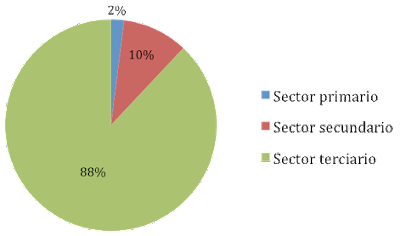
\includegraphics[width=0.5\textwidth]{Memoria_TFG_LaTeX/images/sectoresEconomicosCanarias.png}
    \caption{Distribución de la masa de trabajadores entre los diferentes sectores laborales en Canarias en el año 2020\cite{sectoresEconomicosCanarias}.}
    \label{fig:sectoresCanarias}
\end{figure}

Y en el siguiente diagrama, se observa el aporte del turismo al PIB\footnote{\textbf{PIB}:El producto interior bruto, o por sus siglas PIB, mide la producción total de bienes y servicios de un país. El PIB, por lo tanto, mide el tamaño de la economía de un país, es decir, toda su riqueza económica. Cuánto mayor es el PIB de un país, mayor es su capacidad económica y, por tanto, mayor es su capacidad para generar empleo e inversión.} canario.
\begin{figure}[H]
    \centering
    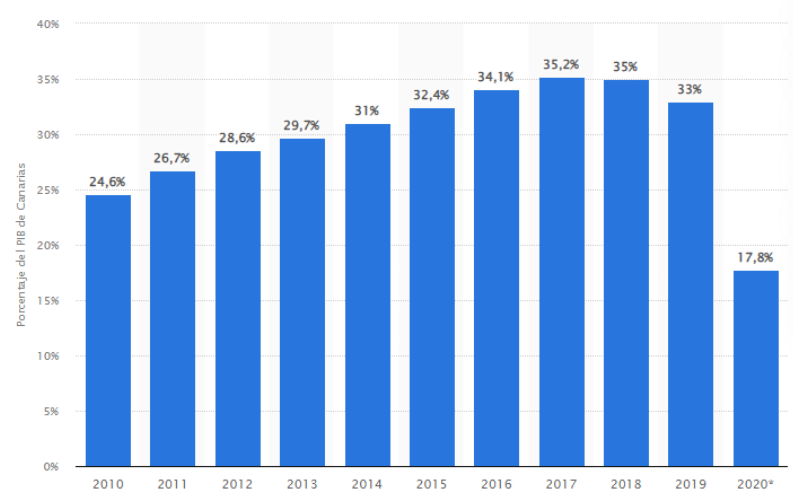
\includegraphics[width=0.5\textwidth]{Memoria_TFG_LaTeX/images/pibcanarias2010-2020.PNG}
    \caption{Aporte del turismo al PIB de canarias. \cite{PIBTurismoCanarias2010-2020}}
    \label{fig:PIB2010-2020}
\end{figure}

Durante los años de pandemia, ha habido un acentuado descenso en la cantidad de turistas que recibe el archipiélago canario. Se estima en un 88.33\% aproximadamente entre 2019 y 2020. 


Afortunadamente, actualmente nos encontramos en un periodo de recuperación económica. 
\begin{figure}[H]
    \centering
    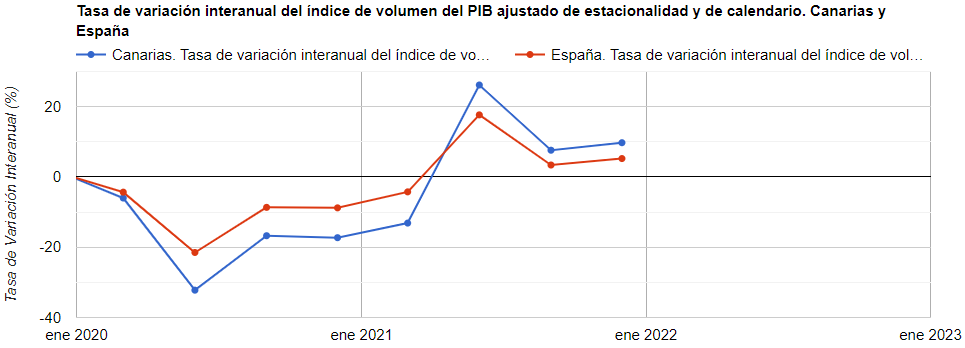
\includegraphics[width=1\textwidth]{Memoria_TFG_LaTeX/images/variacionPIB2020-2022.PNG}
    \caption{Variación del PIB canario entre los años 2020 y 2022. \cite{PIBInteranualCanarias2020-2022}}
    \label{fig:PIB2020-2022}
\end{figure}

Este proyecto pretende dar una motivación más tanto a turistas como a residentes para visitar los diferentes puntos de la Isla y así generar un mayor movimiento turístico en la zona.

%\href{http://www.gobiernodecanarias.org/istac/jaxi-istac/tabla.do?uripub=urn:uuid:ccdf465c-2230-421d-99f6-d6a1669d6032&uripx=urn:uuid:a4f8d3ed-fffc-4f58-b0bf-6ea6d2ab3d54}{info}

%\href{https://docs.google.com/spreadsheets/d/1GL6-trFgfcL-_D5phbUSWi1dCoglB_obWns4Yj6WN9Q/edit#gid=1515882426}{GoogleSheet}

\section{Justificación}

Esta aplicación puede motivar el turismo por la Isla de dos maneras:
\begin{itemize}
\item La primera es promocionando los sitios turísticos que se encuentran cerca del usuario, funcionando como una guía turística convencional, pero con las ventajas que la plataforma móvil ofrece, como pueden ser, la disponibilidad, la actualización constante de contenido, la portabilidad, etcétera.

\item La segunda es el entretenimiento que ofrece con la parte ludificada del proyecto. El mundo de los videojuegos está repleto de premios y logros que van recompensando al jugador por su curiosidad, interés y en definitiva, por seguir jugando \cite{porquenosgustanvideojuegos}. La aplicación presentada podría hacer que aquellos usuarios que sean coleccionistas que buscan completar todos esos premios intentasen completar el mapa de Tenerife, volviendo a generar movimiento por la Isla.

\end{itemize}

Otro factor importante que puede justificar el proyecto es promover el consumo de productos o servicios de kilómetro cero\footnote{\textbf{Producto de kilómetro cero}: Los alimentos, productos o servicios de kilómetro cero son aquellos elaborados a menos de 100 km del punto de venta.} como con las numerosas ventajas que ofrece este tipo de consumo. \cite{kilometro0} Como se comentará más adelante, sería posible incluir publicidad de establecimientos locales cercanos, como pueden ser restaurantes típicos como los denominados guachinches\footnote{\textbf{Guachinche}: es un establecimiento propio de la zona norte de la isla de Tenerife, en el que se ofrece comida casera tradicional, como acompañamiento al vino de cosecha propia o de la zona a precio reducido por ser comprado directamente al productor es este.} o tiendas de artesanía típica canaria, etc. De esta forma, se favorecería un turismo orientado al consumo local, que ayudaría a las pequeñas empresas locales y al disfrute de toda la naturaleza de la Isla. Gracias a tener acceso al GPS\footnote{\textbf{GPS}: Sistema de Posicionamiento Global (Global Positioning System) es un sistema que permite posicionar cualquier objeto sobre la tierra con una precisión de metros o incluso de centímetros.} del dispositivo del usuario este tipo de publicidad sería mucho más efectiva y mejor dirigida.

En los últimos años, este tipo de turismo parece haber aumentado en proporción al turismo más típico de "todo incluido"\cite{turismotodoincluido}. También durante los últimos años, el Gobierno de Canarias ha lanzado varias campañas para promover el cambio de modelo de turismo a uno en el que se consuman más productos locales \cite{campañaelaboradoencanarias}.

\section{Tendencia de mercado}
Como se ha comentado anteriormente, en la actualidad, nos encontramos en un periodo de recuperación turística de suma importancia. Ya que, durante los años de restricciones por la pandemia de Covid 19, el flujo de turistas se redujo prácticamente a cero. En el siguiente gráfico podemos observar ese descenso brusco del número de turistas durante los años 2020 y la recuperación de ese flujo de turistas durante el año 2021 en adelante.

\begin{figure}[H]
    \centering
    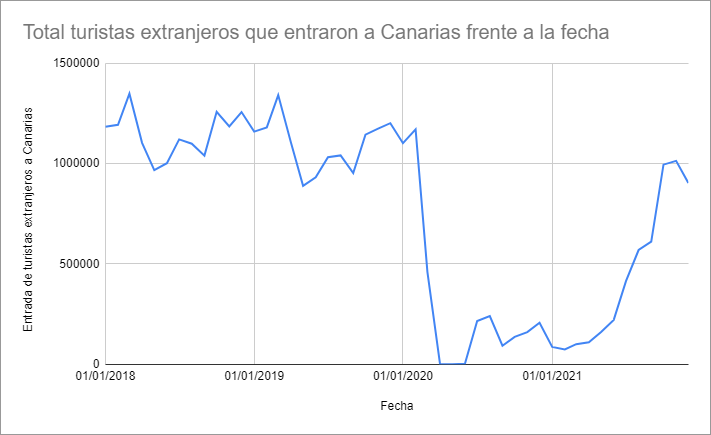
\includegraphics[width=1\textwidth]{Memoria_TFG_LaTeX/images/turistas2018-2022.png}
    \caption{Gráfico que muestra la entrada de turistas extranjeros a Canarias por año.}
    \label{fig:turistas}
\end{figure}

Se puede apreciar que se está comenzando a recuperar el nivel prepandémico.
Con lo cual, el año actual es el momento óptimo para lanzar una aplicación destinada a fortalecer el turismo, pues éste está en pleno auge a niveles prepandémicos.

\section{Estado actual y competencia}
Hoy en día, en la Google Play Store\footnote{\textbf{Google Play Store}:  Anteriormente llamado Android Market, es una plataforma de distribución digital de aplicaciones móviles para los dispositivos con sistema operativo Android, así como una tienda en línea desarrollada y operada por Google. Esta plataforma permite a los usuarios navegar y descargar aplicaciones (desarrolladas mediante Android SDK), juegos, música, libros, revistas y películas.} podemos encontrar varias guías turísticas. 
La mayoría de estas están en formato Ebook\footnote{\textbf{Ebook}: Se trata de una versión digitalizada de un libro, algunos Ebooks no tienen edición física.} lo que impide una mayor interacción por parte del usuario. Como los libros de guías turísticas tienen mayor tiempo en el mercado, estos poseen mayor prestigio o confianza a la vista de un usuario medio. Pero, por contraparte, este tipo de guías son más difíciles de actualizar con nuevos puntos de interés.
Ya existen algunas aplicaciones que hacen de guía turística disponibles en la plataforma, pero ninguna de ellas posee ese factor de gamificación o de recompensa al usuario por visitar esos lugares, más allá del disfrute del propio lugar. A continuación, se muestra una tabla que analiza las diferencias, ventajas y desventajas de las otras guías ya disponibles en comparación con mi propuesta.

\begin{ThreePartTable}
\label{table:competencia}
\captionof{table}{Comparativa del prototipo de DiscoverTenerife con la competencia}

\begin{tabularx}{0.9\textwidth} { 
  | >{\centering\arraybackslash}X 
  | >{\centering\arraybackslash}X
  | >{\centering\arraybackslash}X
  | >{\centering\arraybackslash}X
  | >{\centering\arraybackslash}X | }
 \hline
 Nombre & Ventajas & Desventajas & Similitudes & Diferencias\\
 \hline\hline
 Ebooks & Más experiencia y más renombre & De pago, no interactiva, solo lectura & Señala lugares de interés & No gamificada y no interactiva\\
\hline
Tenerife Guia Turística & Muy buenas valoraciones en Google Play Store, opciones para reservar en villas y hoteles, tiene navegador GPS interno para llegar a los lugares & No parece recordar si se ha visitado un lugar o no & Señala lugares de interés & Mi prototipo solamente incluirá parajes naturales o lugares públicos, no gamificado\\
\hline
Mapa de Tenerife offline + guía & Buenas valoraciones en Google Play Store funciona sin conexión a internet, tiene descripciones de cada ubicación & No parece recordar si se ha visitado un lugar o no & Señala lugares de interés & No gamificado, en la versión premium tiene sistema de navegación GPS, sistema de ubicaciones favoritas \\
\hline
Tenerife: Guía de viaje & Base de usuarios en Google Play Store & No parece recordar si se ha visitado un lugar o no & Señala lugares de interés & No gamificado, permite planificar visitas de varios días, incluye restaurantes, hoteles y tours \\
\hline
\end{tabularx}

\end{ThreePartTable}
\section{Objetivos}
Este estudio pretende responder a las siguientes preguntas: ¿Es rentable una aplicación móvil de guía turística ludificada con estas características? ¿Ayudará realmente a incrementar el turismo por la zona?

Para responder a esas preguntas se han planteado los siguientes objetivos:

\begin{itemize}

\item Analizar las herramientas software o tecnologías disponibles para llevar a cabo el desarrollo y seleccionar la más adecuada o conveniente.

\item Identificar la competencia y establecer una serie de características con las que destacar nuestro proyecto frente a las otras soluciones disponibles.

\item Desarrollo de arquitecturas:

    \begin{itemize}
    
    \item Desarrollar un Web Scraper que capture la información de los puntos de interés.
    
    \item Implementar aplicación en Android.
    
    
        \begin{itemize}
        
        \item Se muestran los puntos de interés más cercanos a la ubicación actual del usuario.
        
        \item Se detecta cuando un usuario ha visitado un punto de interés.
        
        \item Existen opciones para permitir que el usuario decida que puntos de interés ver.
        
        \item Existen opciones para permitir al usuario elegir como se ordenan los puntos de interés; de menor distancia a mayor o de más visitados por el conjunto de usuarios, a menos visitados.
        
        \end{itemize}
        
    
    \item Desarrollar Backend con el que conectará dicha aplicación.
    
        \begin{itemize}
            
        \item El usuario puede registrarse con email y contraseña o de forma anónima.
        
        \item La información relativa al usuario es almacenada en el servidor: qué lugares ha visitado y cuando.
        
        \item La información relativa a los puntos de interés es almacenada en el servidor: nombre, dirección, coordenadas geográficas, etc.
        
        \end{itemize}
    
    \item Desarrollar una página web sencilla que permita consultar la tabla de clasificación de los usuarios.
    
    \end{itemize}
\item Realizar las pertinentes pruebas al conjunto de la aplicación.

\item Desarrollar un plan de negocio para la comercialización del producto:

    \begin{itemize}
    
    \item Crear un Diagrama de Gantt\footnote{\textbf{Diagrama de Gantt}: es una herramienta gráfica cuyo objetivo es exponer el tiempo de dedicación previsto para diferentes tareas o actividades a lo largo de un tiempo total determinado. No muestra las relaciones entre las diferentes tareas.} con las tareas a realizar, su duración, sus recursos y su costo.
    
    \item Prever la inversión inicial del proyecto.
    
    \item Diseñar modelo de comercialización del producto.
    
    \item Calcular el ROI\footnote{\textbf{ROI}: El retorno sobre la inversión (ROI, por las siglas en inglés de return on investment) es una métrica financiera que compara el beneficio o la utilidad obtenida en relación con la inversión realizada, es decir, calcula a partir de qué punto un proyecto comienza a ser rentable recuperando el dinero invertido, tanto al comienzo como durante el proceso.}.
    
    \end{itemize}
    
\end{itemize}





%%%%%%%%%%%%%%%%%%%%%%%%%%%%%%%%%%%%%%%%%%%%%%%%%%%%%%%%%%%%%%%%%%%%%%%%%%%%%%%
\newpage{\pagestyle{empty}}
\thispagestyle{empty}

\chapter{\LARGE Estudio previo}
\label{chapter:estudioPrevio}

En esta sección se explicarán las diferentes tecnologías o herramientas que se han barajado como opciones a la hora de desarrollar el proyecto. Además, se concretará con qué tecnologías o herramientas se ha llevado a cabo finalmente el desarrollo del proyecto.

\section{Lenguaje de programación}
Hoy en día, cada vez más aplicaciones de Android se desarrollan en Kotlin\footnote{\textbf{Kotlin}: es un lenguaje de programación de tipado estático que corre sobre la máquina virtual de Java y que también puede ser compilado a código fuente de JavaScript.}, con lo cual, poco a poco le está quitando terreno al anterior líder del sector Java\footnote{\textbf{Java}: Es un lenguaje de programación, la principal característica de Java es que es compilado a bytecode y luego, es ejecutado interpretándose en una máquina virtual, con lo cual, los programas Java únicamente se compilan una vez, aunque estos se ejecuten en diferentes sistemas.}\cite{kotlinPreferidoPorGoogle}. Los siguientes lenguajes más utilizados son JavaScript\footnote{\textbf{JavaScript}: es un lenguaje de programación interpretado. Se define como orientado a objetos, basado en prototipos, imperativo, débilmente tipado y dinámico. Se utiliza principalmente en navegadores web, permite mejoras en la interfaz de usuario y páginas web dinámicas.} y C\#\footnote{\textbf{C\#}: es un lenguaje de programación multiparadigma desarrollado y estandarizado por la empresa Microsoft como parte de su plataforma .NET}. A continuación se compararán los beneficios y defectos de cada uno de los lenguajes.

\begin{itemize}

    \item \textbf{Kotlin}: De sintaxis sencilla y moderna, se ejecuta en una máquina virtual de Java\footnote{\textbf{Máquina virtual de Java}: Es una máquina virtual ejecutable en una plataforma específica, capaz de interpretar y ejecutar instrucciones expresadas en el bytecode Java, el cual es generado por el compilador del lenguaje Java.}, con lo que permite que los programas se ejecuten en cualquier plataforma que posea esta máquina virtual.
    \begin{itemize}
        \item Ventajas: Multiplataforma.
        \item Desventajas: Carezco de experiencia en Kotlin.
    \end{itemize}
    
    \item \textbf{Java}: Algo más complejo que Kotlin, pero al igual que Kotlin, se ejecuta en una máquina virtual de Java.
    \begin{itemize}
        \item Ventajas: Multiplataforma.
        \item Desventajas: Carezco de experiencia en Java.
    \end{itemize}
    
    \item \textbf{JavaScript}: Potente lenguaje ampliamente utilizado en páginas web, puede usarse para crear apps en Android utilizando React Native\footnote{\textbf{React Native}: Es un proyecto de código abierto especializado en la creación de interfases de usuario. Esta plataforma permite desarrollar aplicaciones para los principales sistemas operativos, tanto móviles como de sobremesa, utilizando el entorno de desarrollo de React con las compatibilidades nativas del sistema.}.
    \begin{itemize}
        \item Ventajas: Multiplataforma, poseo experiencia en JavaScript. 
        \item Desventajas:
    \end{itemize}
    
    \item \textbf{C\#}: Permite crear aplicaciones multiplataformas, el mismo código se puede exportar para iOS, Android y Windows.
    \begin{itemize}
        \item Ventajas: Multiplataforma, poseo experiencia en C\#. 
        \item Desventajas:
    \end{itemize}

\end{itemize}

\section{Entorno de desarrollo}
Para elegir el entorno de desarrollo se han comparado los siguientes frameworks:

\begin{itemize}
\item \textbf{Unity}: pese a ser un motor de desarrollo de videojuegos, presenta utilidades y herramientas que facilitan el desarrollo de una app de estas características, como pueden ser la facilidad para exportar el proyecto a diferentes plataformas.

\item \textbf{Android Studio}: es el entorno de desarrollo integrado oficial para la plataforma Android. Fue creado específicamente para crear aplicaciones en Android.

\item \textbf{Microsoft Visual Studio}: es compatible con múltiples lenguajes de programación, permite a los desarrolladores crear sitios y aplicaciones web, así como servicios web en cualquier entorno compatible con la plataforma .NET.

\item \textbf{Visual Studio Code}: es un editor de código fuente desarrollado por Microsoft. Incluye soporte para la depuración, control integrado de Git, resaltado de sintaxis, finalización inteligente de código, fragmentos y refactorización de código.
\end{itemize}

\section{Plataforma para el backend}
En cuanto al backend se han valorado las siguientes opciones:

\begin{itemize}
\item \textbf{Firebase}: es una plataforma para el desarrollo de aplicaciones web y aplicaciones móviles, está alojada en la nube y permite a los desarrolladores: sincronizar fácilmente datos de usuarios, usar herramientas multiplataformas, usar la infraestructura de Google, la cual, escala automáticamente, autentificación de usuarios, almacenamiento en la nube, etc. Todas estas ventajas abstraen al desarrollador de la parte compleja del desarrollo de un servidor. Es gratuito hasta cierto límite de usuarios.

\item \textbf{Heroku}: es una plataforma de computación en la nube que soporta distintos lenguajes de programación. Para usarlo, habría que elegir JavaScript como lenguaje de programación porque no es compatible con C\#. 
\end{itemize}

\section{Elección final del entorno de desarrollo}
Finalmente, para el desarrollo del grueso del proyecto, se ha decidido utilizar las siguientes herramientas:
\begin{itemize}
\item \textbf{Lenguaje de programación}: C\#.
\item \textbf{Entorno de desarrollo}: Unity y Visual Studio Code.
\item \textbf{Backend}: Firebase.
\item \textbf{Control de versiones}: Git\footnote{\textbf{Git}: es un software de control de versiones pensando en la eficiencia, la confiabilidad y compatibilidad del mantenimiento de versiones de aplicaciones. Su propósito es llevar registro de los cambios en archivos, incluyendo coordinar el trabajo que varias personas realizan sobre archivos compartidos en un repositorio de código.} y Github\footnote{\textbf{GitHub}: es una plataforma de desarrollo colaborativo para alojar proyectos utilizando el sistema de control de versiones Git. Se utiliza principalmente para la creación de código fuente de programas de ordenador.}.
\end{itemize}
Principalmente, se han elegido esas herramientas porque resultan adecuadas para el desarrollo del proyecto y además he trabajado previamente en ellas.

Cabe destacar que para la creación del web scraper se ha utilizado Python\footnote{\textbf{Python}: es un lenguaje de programación interpretado cuya filosofía hace hincapié en la legibilidad de su código. Es un lenguaje interpretado, dinámico, orientado a objetos y multiplataforma.} y la librería Selenium\footnote{\textbf{Selenium}: es un entorno de pruebas de software para aplicaciones basadas en la web. Permite automatizar pruebas para comprobar la interfaz de usuario de una página web.}. También se ha utilizado Python para generar un script que señala los lugares de interés repetidos para su posterior tratamiento manual y JavaScript para añadir a los puntos de interés qué zona de la isla de Tenerife pertenecen, ya que esto se hizo a posterior de tener la información de todos los puntos de interés.

\section{Elección de herramientas para generar la documentación}
La memoria del proyecto ha sido generada con \LaTeX{}\footnote{\textbf{Latex}: es un lenguaje de marcado que permite la composición de textos. Está especialmente orientado a la creación de documentos escritos que presenten una alta calidad tipográfica. Por sus características y posibilidades, es usado asiduamente en la generación de artículos y libros científicos.} utilizando la herramienta en línea \href{http://www.overleaf.com}{Overleaf}\footnote{\textbf{Overleaf}: es una aplicación web que permite, escribir, editar y publicar textos científicos escritos con \LaTeX{}}.
Y, por otro lado, la documentación del código fuente de la aplicación ha sido generada con la herramienta gráfica de \href{https://www.doxygen.nl/index.html}{Doxygen}\footnote{\textbf{Doxygen}: es un generador de documentación para C++, C, C\# y Java, entre otros. Dado que es fácilmente adaptable, funciona en la mayoría de sistemas Unix, así como en Windows y Mac OS X.}.


%%%%%%%%%%%%%%%%%%%%%%%%%%%%%%%%%%%%%%%%%%%%%%%%%%%%%%%%%%%%%%%%%%%%%%%%%%%%%%%
\newpage{\pagestyle{empty}}
\thispagestyle{empty}

\chapter{\LARGE Desarrollo de estructuras}
\label{chapter:desarrolloEstructuras}

\section{Código fuente del web scraper}
El web scraper que ha rastreado internet para extraer la información de los lugares de interés ha sido programado en Python utilizando la librería Selenium.

Su código fuente es un script sencillo con el que se simula que un usuario está navegando por internet con el navegador de Google Chrome. Pero, básicamente, este ha buscado en Google Maps y ha recolectado la siguiente información de cada lugar:

\begin{itemize}
    \item Nombre.
    \item URL de la foto.
    \item Dirección.
    \item Coordenadas geográficas.
\end{itemize}

Toda la información recolectada la ha almacenado en un fichero de texto plano separado por carpetas llamadas igual que las categorías que se han establecido.

Además, he programado otro script, en Python, que realiza las siguientes operaciones:
\begin{itemize}
    \item Descarta los sitios que tengan el mismo nombre dentro de la misma categoría, ya que presumiblemente serán el mismo lugar.
    \item A cada lugar le asigna la zona de la isla, de las que se han definido dentro de la aplicación, que le corresponda por sus coordenadas geográficas. Las divisiones en zonas de la isla será definida en su propia sección dentro del quinto capítulo.
    \item Genera un fichero en formato JSON con los sitios que aparecen en más de una categoría. Estos deben ser revisados manualmente.
    \item Genera un fichero en formato JSON con el resto de sitios, dividiéndolos por categoría.
\end{itemize}

\section{Estructura código fuente de la aplicación}
Para el desarrollo del código fuente de la aplicación se ha seguido el paradigma de programación orientado a objetos y también se ha hecho uso de eventos, ya que este es el modelo con el que trabaja Unity. Además, para cada pantalla se han utilizado diferentes escenas, las cuales serán explicadas a continuación.

\subsection{Escenas}
Los proyectos de Unity son, comúnmente, divididos en escenas. Para desarrollar DiscoverTenerife se ha seguido ese patrón de escenas independientes con algunos objetos que permanecen entre escenas para conservar información, como es el caso de firebaseHandler o gpsController. 

Las escenas en las que se ha dividido el proyecto coinciden con las diferentes pantallas que nos encontramos en la aplicación:

\begin{itemize}
\item \textbf{Login}: Pantalla sencilla con 5 botones que dirigen a los diferentes métodos de inicio de sesión o de registro. Tenemos las siguientes opciones que nos dirigen a otras pantallas: 
\begin{itemize}
    \item \textbf{Sign In}: Para iniciar sesión mediante correo y contraseña, debemos tener una cuenta previamente creada.
    
    \item \textbf{Register}: Para registrarse como nuevo usuario mediante correo y contraseña.
    
    \item \textbf{Iniciar sesión con Google}: Para iniciar sesión utilizando la autenticación de Google, debemos tener una cuenta previamente creada con Google para acceder de esta forma.
    
    \item \textbf{Registrarse con Google}: Para crear una cuenta utilizando la autenticación de Google.
    
    \item \textbf{Inicio de sesión anónimo}: Para iniciar sesión utilizando la de usuario anónimo de firebase. Este sistema ha sido incluido para usuarios que solo quieran utilizar la aplicación como una guía turística convencional, sin utilizar factores competitivos o sociales. Este tipo de cuentas no están recomendadas porque están ligadas al dispositivo, es decir, si se cambia de dispositivo, se desinstala la aplicación o se borran los datos de la aplicación, se perderá todo el progreso dentro de la aplicación.
\end{itemize}

\item \textbf{Principal}: En esta pantalla encontramos diferentes elementos, un botón que nos llevará a la sección de ajustes, un texto que nos indica en qué zona de la Isla estamos y dos barras de experiencia, una indica el porcentaje de lugares visitados dentro de la zona actual y el otro indica el porcentaje de lugares visitados de todo Tenerife.

Además, se nos mostrarán una serie de lugares en un panel que es deslizable, si deslizamos hacia arriba lo suficiente recargaremos la escena consiguiendo que actualice la lista de lugares teniendo en cuenta nuestra ubicación actual. 

En cambio, si deslizamos hacia abajo, se irán mostrando nuevos lugares ordenados según las preferencias que se hayan definido en la pantalla de ajustes, las cuales serán explicadas más adelante. Se mostrarán hasta 15 lugares, si seguimos deslizando hacia abajo, hasta cierto punto, conseguiremos que la escena recargue teniendo en cuenta que ya hemos visto esos 15 lugares, por lo tanto, tras la recarga se nos mostrarán los siguientes 15 puntos de interés ordenados de nuevo por los ajustes que hayamos decidido.

Si pinchamos sobre alguno de los lugares que se nos ofrecen accederemos a la pantalla de ese lugar, esta pantalla será explicada a continuación.

\begin{figure}[H]
    \centering
    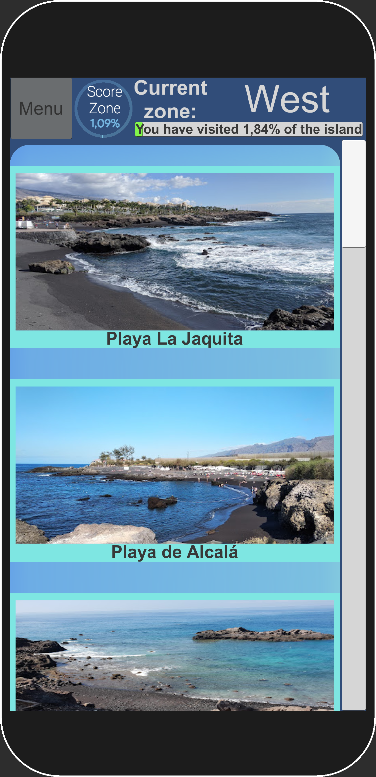
\includegraphics[width=0.25\textwidth]{Memoria_TFG_LaTeX/images/pantallaPrincipal.PNG}
    \caption{Demostración de cómo es la pantalla principal.}
    \label{fig:pantallaPrincipal}
\end{figure}

\item \textbf{Lugar}: En esta pantalla se nos presentará toda la información relativa al lugar: 
    \begin{itemize}
    \item Un cartel que indica si lo hemos visitado previamente o no.
    
    \item Una foto.
    
    \item El nombre, la distancia al usuario, calculada accediendo al sistema de geolocalización del dispositivo del usuario y la dirección, si la dirección no estuviera disponible, se presentarían las coordenadas geográficas exactas de ese punto de interés.
    
    \item Una barra que cambia de color de verde a rojo y de relleno de izquierda a derecha en función de la cantidad de visitas que tenga ese lugar comparado con el resto de lugares.
    
    \item Por último, encontramos 4 botones:
        \begin{itemize}
            \item \textbf{Google Maps}: Abre la aplicación de Google Maps con las coordenadas del punto de interés marcadas en el mapa.
            
            \item \textbf{Retar a un amigo}: Abre una pantalla que nos muestra los amigos que tenemos y se da la opción de retarles a visitar este sitio, siempre y cuando, ese amigo no tenga ya un reto nuestro y haya pasado al menos 7 días desde el último reto que le hayamos enviado.
            
            \item \textbf{Guardar el lugar para una visita sin conexión a Internet}. Podremos guardar hasta 5 lugares para visitar sin conexión.
            
            \item \textbf{Registrar este lugar como visitado}: Si el usuario está suficientemente cerca, al menos a 50 km, y ha cumplido el tiempo de enfriamiento, de 1 hora de tiempo real, se registrará el lugar como visitado y el usuario ganará puntos.
        \end{itemize}
    \end{itemize}

\begin{figure}[H]
    \centering
    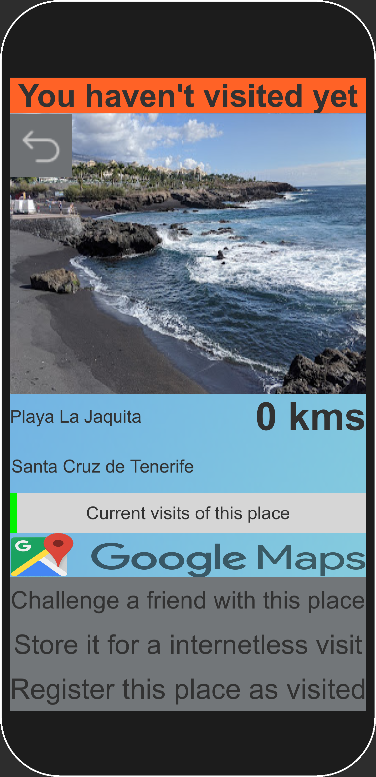
\includegraphics[width=0.25\textwidth]{Memoria_TFG_LaTeX/images/pantallaLugar.PNG}
    \caption{Demostración de cómo se ve la pantalla de un lugar cuando el usuario no lo ha visitado.}
    \label{fig:pantallaLugarNoVisitado}
\end{figure}

\begin{figure}[H]
    \centering
    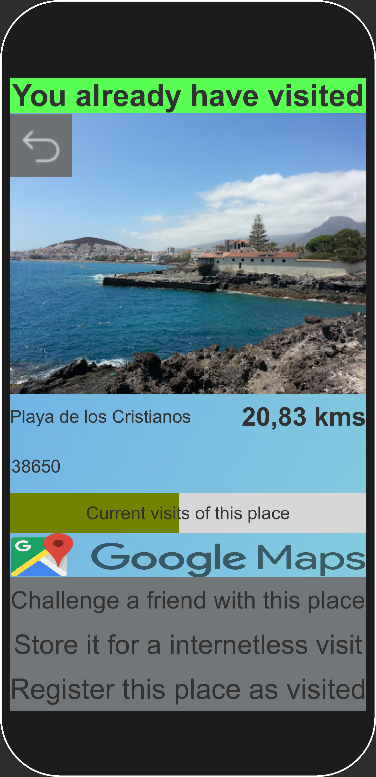
\includegraphics[width=0.25\textwidth]{Memoria_TFG_LaTeX/images/pantallaLugarVisitado.PNG}
    \caption{Demostración de cómo se ve la pantalla de un lugar cuando el usuario lo ha visitado.}
    \label{fig:pantallaLugarVisitado}
\end{figure}

\item \textbf{Menú}: En esta escena se nos muestran una serie de botones que nos llevan a otras pantallas que nos permiten hacer lo que su nombre indica. Las opciones disponibles son:

\begin{itemize}
    
    \item \textbf{Historial de sitios visitados}: pantalla que muestra la lista de lugares que ha visitado el usuario.
    
    \item \textbf{Ranking de jugadores}: pantalla que muestra la lista de jugadores que permiten aparecer en el ranking ordenado por puntuación.
    
    \begin{figure}[H]
    \centering
    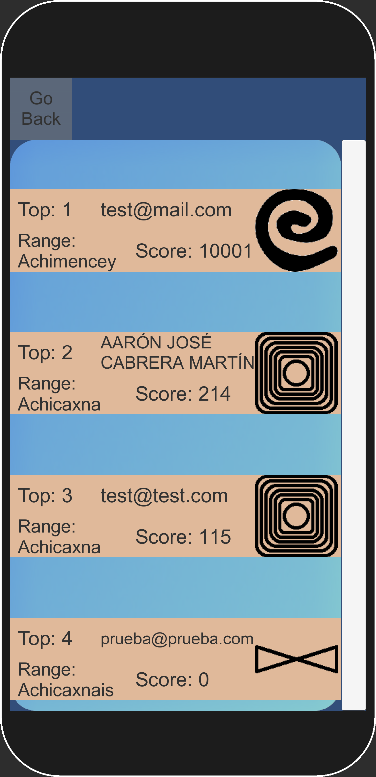
\includegraphics[width=0.25\textwidth]{Memoria_TFG_LaTeX/images/pantallaRanking.PNG}
    \caption{Demostración de cómo se ve la pantalla del ránking.}
    \label{fig:pantallaRanking}
    \end{figure}
    
    \item \textbf{Mi rango y puntuación}: pantalla que muestra nuestro rango, con su respectivo icono y puntuación actual. También se muestra la fecha en la que hemos ascendido a los anteriores rangos.
    
    \item \textbf{Mis estadísticas}: pantalla que muestra el porcentaje de lugares visitados de cada zona de la Isla por separado que llevamos. También se nos muestra la cantidad de lugares diferentes que hemos visitado, la cantidad de visitas acumuladas y el lugar, la zona y el tipo de lugar que más hemos visitado.
    
    \item \textbf{Mis amigos}: pantalla que muestra la lista de amigos que tenemos. Desde aquí podemos retar a un amigo a visitar algún lugar que hayamos guardado anteriormente o eliminar a ese amigo.
    
    \item \textbf{Nuevas invitaciones a amigo}: pantalla que muestra una lista de solicitudes de amistad. Desde esta pantalla podemos, eliminar esa invitación o aceptarla.
    
    \item \textbf{Buscar un nuevo amigo}: pantalla que nos muestra una barra de búsqueda. Si escribimos en ella, se nos mostrarán aquellos jugadores que en su nombre contengan la cadena que hemos escrito y que hayan permitido que otros jugadores les envíen invitaciones de amistad.
    
    \item \textbf{Lugares guardados para una visita sin internet}: en esta pantalla se nos muestra la lista de lugares que tenemos guardado para visitar cuando no tengamos conexión a internet, podemos intentar visitar ese lugar o eliminarlo. Cabe recordar, que para visitar el sitio, seguiremos necesitando la geolocalización. Las visitas que realizamos de esta manera serán subidas al servidor desde que tengamos conexión a internet.
    
    \begin{figure}[H]
    \centering
    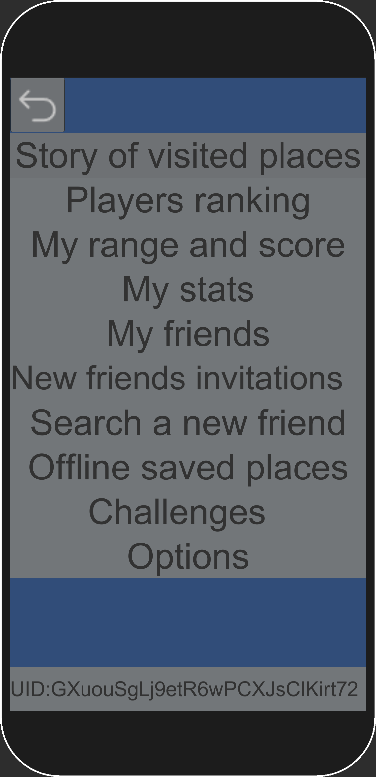
\includegraphics[width=0.25\textwidth]{Memoria_TFG_LaTeX/images/pantallaMenu.PNG}
    \caption{Demostración de cómo se ve la pantalla del menú.}
    \label{fig:pantallaMenu}
    \end{figure}
    
    \item Opciones: en esta sección podremos configurar:
    \begin{itemize}
        \item \textbf{Unidad de medida de la distancia}: kilómetros o millas.
        
        \item \textbf{Tipos de lugares} que queremos encontrar o si deseamos ver lugares ya visitados. Si marcamos que no queremos ver lugares ya visitados, estos tendrán la prioridad mínima al elegir los lugares que se muestran en la pantalla principal.
        
        \item \textbf{Reglas para ordenar los lugares}: si, por menor distancia a tu ubicación o por menor número de visitas del lugar.
        
        \item \textbf{Opciones sociales}: En este apartado podremos elegir si deseamos aparecer en el ranking de usuarios, si deseamos permitir que otros usuarios nos envíen peticiones de amistad y si deseamos permitir que otros amigos nos envíen retos.
        
        \item \textbf{Cerrar sesión}: Con este botón podremos cerrar sesión y volver a la pantalla de inicio de sesión o creación de cuenta.
        
        \item \textbf{Reportar un error}: Si pulsamos este botón se nos abrirá la aplicación de correo electrónico por defecto, por ejemplo, Gmail con un correo preparado, con un texto indicando al usuario que describa lo que ha ocurrido y avisándole de que si puede añadir una captura de pantalla el reporte será mucho más útil.
        
    \end{itemize}
\end{itemize}


\end{itemize}

\subsection{Clases Principales}
\begin{itemize}
\item \textbf{firebaseHandler}: Se encarga de manejar todos los eventos o funciones relacionadas con la base de datos Firebase, el backend de la aplicación. Esta clase ha sido divida en varios ficheros con clases parciales para facilitar su lectura.
Las clases parciales que he realizado han sido:
\begin{itemize}
    \item \textbf{firebaseHandler}: Se trata de la parte principal, se encarga de controlar cuando se puede subir o descargar la información desde el servidor, teniendo en cuenta el estado actual de la conexión a internet. Si no hay conexión a internet, genera una serie de colas que almacenan qué cambios se deben subir para que, desde que se consiga una conexión estable, se suba toda esa información.
    
    \item \textbf{loginHandler}: Encargado de todo el sistema de login de usuarios y registro de nuevos usuarios.
    
    \item \textbf{downloadHandler}: Contiene todos los métodos que descargan información del servidor.
    
    \item \textbf{uploadHandler}: Contiene todos los métodos que suben información al servidor.
    
\end{itemize}

Es decir, el conjunto de ficheros que forman la clase firebaseHandler contiene métodos para crear nuevos usuarios o para iniciar sesión con cada uno de los métodos permitidos. Además, almacena la información del usuario cuando este inicia sesión, la información relativa al usuario es almacenada con un objeto de la clase \textbf{UserData}. La instancia de esta clase es única por cada ejecución y permanece entre escenas. FirebaseHandler también contiene una instancia de la clase \textbf{requestHandler} la cual almacena toda la información relativa a los lugares de interés y lleva el control del orden en el que el usuario debe acceder o visualizar estos, teniendo en cuenta las opciones que el usuario ha seleccionado en la correspondiente pantalla.

\item \textbf{UserData}: Es la encargada de almacenar toda la información relativa al usuario una vez ha iniciado sesión. Se almacena el identificador de usuario, los sitios que ha visitado y el nombre que posee.

\item \textbf{Place}: Se encarga de almacenar la información relativa a un punto de interés, por lo tanto, en tiempo de ejecución existirán varias instancias de esta clase. Posee un método para realizar la descarga de la imagen a través de internet.

\item \textbf{gpsController}: Se encarga de gestionar el acceso al sistema GPS del dispositivo. Además, tiene métodos para verificar que los permisos de acceso al sistema GPS han sido concedidos. La instancia de esta clase permanecerá entre la pantalla principal y la pantalla de un lugar concreto.

\item \textbf{optionsController}: Se encarga de almacenar la configuración actual que el usuario ha escogido, también refleja esos cambios en la pantalla de opciones. La instancia de esta clase permanecerá entre la pantalla principal, la pantalla de un lugar concreto, la pantalla de opciones y la pantalla de estadísticas del usuario.

\item \textbf{MapRulesHandler}: Esta clase contiene atributos y métodos únicamente estáticos. No está pensada para ser instanciada, se comporta como un almacén para la información que únicamente variará si se cambia la zona del planeta en la que trabaja la aplicación.

\item \textbf{gameRules}: Esta clase contiene atributos y métodos únicamente estáticos. No está pensada para ser instanciada, se comporta como un almacén de información o funciones relativas a las reglas del juego. Almacena, por ejemplo, cuánto tiempo tiene que pasar entre dos visitas consecutivas a un lugar o las fórmulas que calculan la puntuación que obtiene el usuario al visitar un lugar o al completar un reto, etc.
\end{itemize}

Recordar que la documentación del código fuente se encuentra disponible en el Github Pages del proyecto\cite{doxygenDiscoverTenerife} y que puede ser consultada para obtener unas mejores explicaciones de como funciona el código interno de la aplicación, ya que allí, se encuentra esta información más extensamente explicada. Asi como que el código fuente de la aplicación para Android, de la página web y del web scraper se encuentran disponibles en el repositorio GitHub del proyecto\footnote{\href{https://github.com/AaronJoseCabreraMartin/TFG-DiscoverTenerife}{https://github.com/AaronJoseCabreraMartin/TFG-DiscoverTenerife}}.


\section{Estructuración de la base de datos}

Tras varias iteraciones, se ha decidido dividir la base de datos en dos sectores principales, los lugares y la información de los usuarios. Finalmente, el diseño que se ha llevado a cabo para implementar ha sido el que se presenta a continuación:

\begin{itemize}
\item \textbf{Lugares}: Tiene una entrada por cada tipo de punto de interés: \textbf{Playas}, \textbf{miradores}, \textbf{rutas de senderismo}, \textbf{parques naturales} y \textbf{piscinas naturales}. A su vez, cada una de estas categorías almacena, utilizando un identificador numérico, la información de cada punto de interés. Por lo tanto, la clave primaria de cada punto de interés sería la tupla: tipo de sitio de interés e identificador numérico.

La información almacenada de cada punto de interés es:
\begin{itemize}
    \item \textbf{Dirección}, si el sitio no posee dirección, se rellena el campo con las coordenadas geográficas.
    \item \textbf{Link a la imagen} del lugar, para la futura descarga de la imagen.
    \item \textbf{Latitud} del punto geográfico donde se encuentre el punto de interés.
    \item \textbf{Longitud} del punto geográfico donde se encuentre el punto de interés.
    \item \textbf{Nombre} del lugar.
    \item \textbf{Número de veces} que ha sido visitado.
    \item \textbf{Zona} de Tenerife en la que se encuentra.
\end{itemize}

\item \textbf{Usuarios}: Almacena una entrada por cada usuario. Donde la clave es el UID\footnote{\textbf{UID}: Siglas de User ID, ID es la abreviación de la palabra Identification. Traducido al español significa: Identificador de Usuario} del propio usuario. Se almacena la siguiente información de cada usuario:
    \begin{itemize}
    \item \textbf{Display name}: nombre del usuario.
    \item \textbf{Places Visited}: Lista ordenada cronológicamente por la \textbf{primera} visita que ha realizado dicho usuario a ese lugar. La clave es un identificador numérico que indica el orden cronológico de la primera visita. Por cada entrada de la lista se almacenan los siguientes valores:
        \begin{itemize}
        \item Identificador numérico del lugar.
        \item El tipo del lugar.
        \item Última vez que ese usuario ha visitado ese lugar, para controlar el tiempo de espera entre visita y visita.
        \item Cuántas veces ha visitado ese usuario ese punto.
        \end{itemize}
    \item \textbf{Base Coords}: Coordenadas del lugar en el que el usuario realizó la primera conexión. Estas coordenadas quedan registradas para poder calcular puntuación extra obtenida por visitar lugares que están más lejos de la zona que presumiblemente suele frecuentar.
    
    \item \textbf{Challenges}: Lista que almacena los retos que tiene el usuario. Cada reto almacena: el usuario que envió el reto, el timestamp del momento en el que el reto fue enviado y la información necesaria para diferenciar el lugar; tipo e id.
    
    \item \textbf{EarnedScore}: Entero que almacena la puntuación que el usuario ha conseguido de forma pasiva. En el prototipo actual, la única forma de conseguirla es cuando un amigo completa uno de nuestros retos.
    
    \item \textbf{Friends}: Lista que contiene los uids de aquellos jugadores a los que hemos aceptado como amigo o los cuales nos han aceptado como amigos.
    
    \item \textbf{RangeStory}: Lista que almacena un elemento cada vez que el usuario sube de rango. Se almacena el rango alcanzado y la fecha.
    
    \item \textbf{Score}: Entero que almacena la puntuación actual del usuario.

    \item \textbf{FriendInvitations}: Lista que almacena las peticiones de amistad que nos han enviado otros usuarios y que aún no hemos respondido.
    
    \item \textbf{AcceptedFriendInvitations}: Lista de las peticiones de amistad que hemos enviado y que el usuario destino ha aceptado. Esta lista se vacía cada vez que el usuario se conecta, los user id que aparecen en esta lista son movidos a la lista de Friends.
    
    \item \textbf{DeletedFriends}: Lista de uids de usuarios que eran nuestros amigos, pero que han decidido eliminar la amistad. Esta lista se vaciará en cada login. Todos los user id que se encuentren en esta lista serán eliminados de la lista Friends sin notificar nada al usuario.
    
    \end{itemize}

\item Usuarios que permiten recibir \textbf{peticiones de amistad}: Lista de uids de los usuarios que tienen habilitada la opción de recibir peticiones de amistad de otros usuarios. Si tienen desactivada esa opción, son eliminados de esta lista y, por lo tanto, la única manera que tienen de establecer una amistad es ellos mismos mandar la invitación a otro usuario que sí tenga esa opción activada.

\item Usuarios que permiten aparecer en el \textbf{ránking de usuarios}: Lista de uids de usuarios que tienen habilitada la opción de aparecer en el ránking de usuarios. Si tienen desactivada esta opción, no se les tendrá en cuenta a la hora de calcular las posiciones del ránking de usuarios.

\item Usuarios que permiten \textbf{ser retados por otros usuarios}: Lista de uids de usuarios que tienen activada la opción de que sus amigos les envíen retos. Si tienen esta opción desactivada, cuando alguno de sus amigos intente retarles, directamente no les aparecerá en la lista de usuarios rentables.

\end{itemize}

\subsection{Reglas de seguridad de la base de datos}
Una vez establecida la estructura de la base de datos, el siguiente paso ha sido establecer unas reglas de seguridad apropiadas. Las reglas que se han establecido son:
\begin{itemize}
\item Cualquier petición de un usuario no identificado se rechaza.
\item Todos los usuarios autentificados pueden leer la información de los sitios de interés.
\item Todos los usuarios autentificados pueden sobreescribir el valor de la propiedad ``número de veces visitado`` de todos los sitios de interés.
\item En la parte de usuarios, los usuarios únicamente pueden leer y escribir la información de su propia entrada, excepto las listas de ``acceptedFriends``, ``deletedFriends``, ``earnedScore`` y ``challenges``. Estas listas pueden ser modificadas por cualquier usuario identificado que además no sea anónimo. Esto es así para permitir establecer relaciones de amistad, eliminar relaciones de amistad, retar a otros jugadores u obtener puntuación por haber hecho que un amigo complete uno de tus retos. Se excluye a los jugadores anónimos del permiso de escritura de estas listas porque, estos jugadores no tienen permitido el acceso a las funcionalidades sociales que utilizan estas características. 

\end{itemize}
Con estas reglas, se les permite a los usuarios autentificados leer toda la información de los sitios de interés, pero solamente escribir el único campo que depende de ellos; el número de veces visitado. Y se impide que los usuarios puedan escribir en los campos de otros usuarios, excepto los que son necesarios.

También es importante destacar que en las listas; ``usersThatAllowFriendshipsInvitations``, ``usersThatAllowBeChallenged``, ``usersThatAllowAppearedOnRanking``, en las cuales están apuntados los id de usuario de cada usuario que permite; recibir invitaciones de amistad, ser retado por sus amigos o aparecer en el ránking respectivamente. Cada usuario puede elegir si estar o no en cada una de esas listas en el menú de opciones, por lo tanto, todos los usuarios autentificados pueden añadir o eliminar su uid de cualquiera de las tres listas.

\subsection{Métodos de autenticación}
La gestión de usuarios es otra herramienta que ofrece Firebase, para este proyecto se ha decidido utilizar los siguientes métodos de autentificación:
\begin{itemize}
\item \textbf{Correo electrónico y contraseña}: Introduciendo un correo electrónico y una contraseña de, al menos, seis dígitos de longitud, un usuario puede registrarse e iniciar sesión.
\item \textbf{Inicio de sesión con Google}: Utiliza una sesión iniciada previamente de una cuenta Google del dispositivo, es la opción más segura y recomendada.
\item \textbf{Inicio de sesión anónimo}: Este método que incluye firebase consiste en generar un User ID para esa instancia de ese dispositivo, es decir, si se borra los datos de la aplicación, se desinstala la aplicación y luego se instala de nuevo o si se cambia de terminal móvil, se perderá la información del usuario. Este método, puesto que fácilmente se puede perder el progreso conseguido, solo está recomendado para un primer contacto con la app, o para los usuarios que quieran utilizar la aplicación solamente para descubrir los lugares, como si se tratase de una guía turística tradicional.
\end{itemize}


%%%%%%%%%%%%%%%%%%%%%%%%%%%%%%%%%%%%%%%%%%%%%%%%%%%%%%%%%%%%%%%%%%%%%%%%%%%%%%%
\newpage{\pagestyle{empty}}
\thispagestyle{empty}

\chapter{\LARGE Ludificación del proyecto}
\label{chapter:ludificacion}

\section{Concepto de ludificación}
En este capítulo definiremos qué es la ludificación, también conocida como ``gamificación``\cite{definicionGamificacion} por su anglicismo \textit{gamification}, sus aspectos más importantes y por qué resulta una herramienta útil para incrementar la participación de los usuarios.

La ludificación es el uso de técnicas y elementos propios de los juegos o de los videojuegos en otro tipo de actividades para potenciar la participación y motivación de quienes realizan dichas actividades. Ejemplo de elementos de ludificación serían, puntuaciones, rangos diferenciados de nivel de progreso, tablas de clasificación o división de las actividades en retos que van otorgando recompensas o reconocimientos al trabajo de los participantes, etcétera. Es importante, para que la ludificación tenga éxito, que los usuarios sean conscientes de su progreso. Por ello, se han implementado algunas recompensas que otorgan al usuario una retroalimentación\footnote{\textbf{retroalimentación}: feedback, en inglés, hace referencia a dar información sobre el resultado de una acción, en este caso concreto, para que el usuario sea consciente de que ha obrado bien y ha progresado dentro de la aplicación.} positiva.

El factor competitivo resulta de suma importancia a la hora de incentivar la participación y motivación de los usuarios\cite{caponetto2014gamification}. El hecho de estar en un entorno competitivo hace que las personas se esfuercen por destacar y por mejorar\cite{alsawaier2018effect}. Este fenómeno está relacionado con una necesidad que tiene el ser humano de pertenecer a un grupo ganador o sentir que su esfuerzo tiene valor, pero, no hay que olvidar que esta necesidad se intensifica o se atenúa dependiendo de la personalidad\cite{ghaban2019different}. Aunque, por otra parte, si el individuo no percibe progreso a pesar de su esfuerzo, puede generar sentimientos de frustración\cite{nicholson2015recipe}. Por lo tanto, es importante que en todo momento el usuario sea consciente de que está progresando y superando a otros dentro del sistema de juego establecido.

Por ello, se han creado rangos de poder, tablas clasificatorias y formas de retar a otros usuarios dentro de la aplicación.

En los siguientes apartados se explicará la parte ludificada de la aplicación, es decir, los factores gamificados, las reglas y las recompensas.

\section{Reglas para conseguir puntuación}
Una de las partes más importantes de un juego o de una actividad gamificada, como ya hemos visto, es poder contabilizar y apreciar el progreso. Para que el usuario sea consciente de estos progresos se suelen utilizar puntuaciones cuya obtención se encuentra limitada por una serie de reglas o normas. Ese será el tema que vamos a tratar, a continuación, qué reglas controlan el progreso del jugador:
\begin{itemize}
\item \textbf{Considerar un punto de interés como visitado}: Para que un usuario pueda registrar un punto de interés como visitado, debe estar físicamente a menos de \textbf{50 metros} de ese punto de interés, además, el usuario debe entrar en la aplicación, seleccionar ese punto de interés y tratar de registrar su visita haciendo clic en el botón habilitado para ello. Para calcular la distancia a dicho punto de interés, el usuario debe tener activada la ubicación mediante servicio GPS de su dispositivo móvil y conceder los consecuentes permisos a la aplicación. Conexión a internet no es necesaria porque se ha habilitado una opción de visita offline.
\item \textbf{Tiempo de espera para volver a visitar un punto de interés}: Se ha establecido que para volver a registrar un punto de interés como visitado se debe esperar al menos \textbf{una hora de tiempo real}. 
\end{itemize}

La puntuación asociada a cada acción son las siguientes:
\begin{itemize}
\item 10 puntos por visitar un sitio ya visitado
\item 15 puntos por visitar un sitio no visitado
\item Siempre que se visite un sitio se obtendrá una puntuación extra que será mayor cuanto menos visitado esté ese lugar. Esa puntuación extra se consigue a través de un factor multiplicativo que cumple con la siguiente fórmula:

\begin{displaymath}
2 - \frac{nvl + 1}{nvm + 1}
\end{displaymath}

Donde:
\begin{itemize}
    \item \textbf{nvl}: es Número de Visitas de ese Lugar que se está visitando.
    \item \textbf{nvm}: es Número de Visitas Máximo, es decir, el número de visitas que tiene el lugar más visitado de todos.
\end{itemize}

Nótese que como máximo el factor multiplicativo será casi 2 y como mínimo será 1. Por lo tanto, si visitamos un lugar sin visitas y es la primera vez que lo visitamos, obtendremos 15 * 2, es decir, 30 puntos.

\item Cumplir un reto. Al cumplir un reto, el usuario obtendrá la puntuación descrita en el apartado anterior y además, se le sumará el resultado de la siguiente fórmula:

\begin{displaymath}
(2 - \frac{ct-st}{mt-st})*dub
\end{displaymath}

Donde:
\begin{itemize}
    \item \textbf{ct}: Completation Timestamp, es decir, el momento exacto en el que se está cumpliendo el reto.
    \item \textbf{st}: Start Timestamp, es decir, el momento exacto en el que el reto fue enviado.
    \item \textbf{mt}: Maximum Time, es decir, el plazo máximo que tienen los usuarios para completar un reto.
    \item \textbf{dub}: Distance to User Base, es decir, la distancia en kilómetros que separan la base del usuario del punto que está visitando.

\end{itemize}

Como se puede observar, el resultado será, como máximo, el doble de la distancia en kilómetros a la base del usuario y como mínimo esa distancia exactamente. La fórmula está construida de tal manera que el usuario obtendrá mayor puntuación cuanto más rápido complete el reto y cuanto más lejos de su base se encuentre el punto de interés que está visitando.

\item Cuando un usuario completa un reto, el amigo que le envió ese reto también recibe un pequeño porcentaje del total de la puntuación recibida. Ese porcentaje se ha establecido en un 10\%. 
\end{itemize}

Todos los parámetros y fórmulas referentes a la obtención de puntuación, para facilitar su modificación, están definidos dentro de la clase gameRules.


\section{División de la Isla por zonas dentro de la aplicación}
Hemos decidido dividir la Isla en  \textbf{cinco zonas} o sectores, los cuales, cuatro de ellos, coinciden con los puntos cardinales, Norte, Sur, Este y Oeste. Pero además, se ha añadido un sector central.

Cada zona se ha determinado por las coordenadas geográficas de dicho rectángulo. A continuación, se mostrarán las coordenadas de cada zona:

\begin{ThreePartTable}
\label{table:zonas}
\captionof{table}{División en zonas del mapa de la isla de Tenerife}

\begin{tabularx}{0.9\textwidth} { 
  | >{\raggedright\arraybackslash}X
  | >{\raggedright\arraybackslash}X
  | >{\raggedright\arraybackslash}X
  | >{\raggedright\arraybackslash}X
  | >{\raggedleft\arraybackslash}X | }
    \hline
    Nombre Zona & \multicolumn{2}{|c|}{Esquina inferior izquierda} & \multicolumn{2}{|c|}{Esquina superior derecha}\\
    \hline
    \hline & Latitud & Longitud & Latitud & Longitud\\
    \hline Norte  & 28.40631 & -16.93788 & 28.60634 & -16.11673\\
    \hline Oeste  & 28.14750 & -16.93788 & 28.40631 & -16.67719\\
    \hline Centro & 28.14750 & -16.67719 & 28.40631 & -16.53193\\
    \hline Este   & 28.14750 & -16.53193 & 28.40631 & -16.11673\\
    \hline Sur    & 27.99321 & -16.93788 & 28.14750 & -16.11673\\
    \hline 
\end{tabularx}
\end{ThreePartTable}

Nótese que al tratarse de divisiones rectangulares, solamente con saber las coordenadas de dos esquinas opuestas diagonalmente podemos determinar si un punto está dentro de una zona o no. Para determinar en qué zona de la Isla está cada punto de interés se han utilizado las coordenadas geográficas de dicho punto.

Para facilitar que el usuario sea consciente del progreso que ha llevado en la aplicación, dentro de la ventana del menú, existe la opción de acceder a la pantalla de puntuaciones. En esta pantalla, el usuario verá una imagen de Tenerife con fondo blanco y con las zonas, previamente explicadas, señaladas y enmarcadas dentro de rectángulos rojos.

\begin{figure}[H]
    \centering
    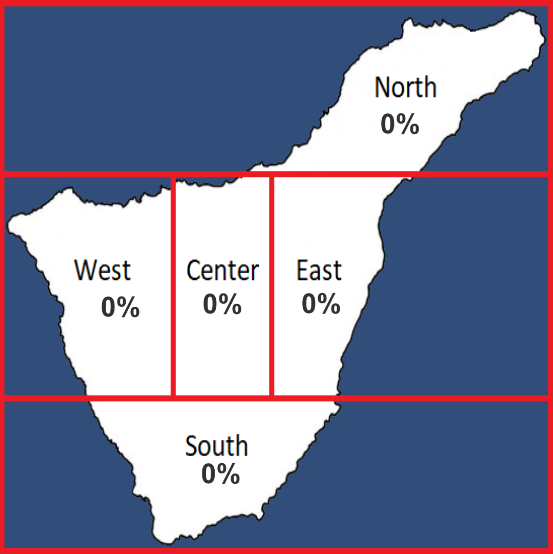
\includegraphics[width=0.25\textwidth]{Memoria_TFG_LaTeX/images/mapaNoCompleto.png}
    \caption{Demostración de cómo se verá el mapa cuando no se haya realizado ninguna visita.}
    \label{fig:mapaNoCompleto}
\end{figure}

Además, las zonas se irán rellenando, proporcionalmente a la cantidad de puntos de interés visitados dentro de esa zona, de un color azul.

\begin{figure}[H]
    \centering
    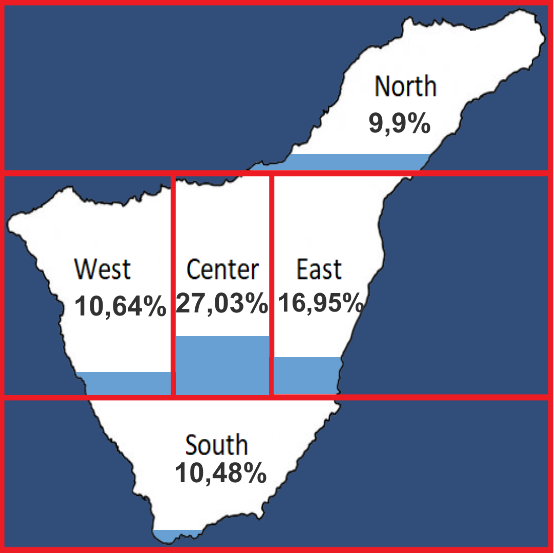
\includegraphics[width=0.25\textwidth]{Memoria_TFG_LaTeX/images/mapaParcial.png}
    \caption{Demostración de cómo se verá el mapa cuando se haya visitado cierta cantidad de puntos de cada zona.}
    \label{fig:mapaParcial}
\end{figure}

\begin{figure}[H]
    \centering
    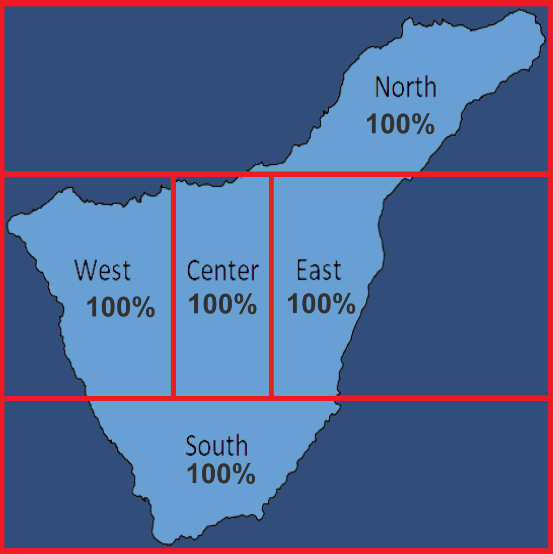
\includegraphics[width=0.25\textwidth]{Memoria_TFG_LaTeX/images/mapaCompleto.png}
    \caption{Demostración de cómo se verá el mapa una vez se hayan visitado todos los puntos de interés de la Isla al menos una vez}
    \label{fig:mapaCompleto}
\end{figure}

En la misma pantalla es posible observar diferentes estadísticas del usuario, como son:
\begin{itemize}
\item Número \textbf{total} de visitas realizadas, contabilizando varias visitas a un mismo punto.
\item Número de puntos de interés \textbf{diferentes} visitados.
\item La \textbf{zona} de la Isla más visitada.
\item El \textbf{tipo} de sitio de interés más visitado
\item El \textbf{sitio} de interés más visitado de todos.
\end{itemize}

\begin{figure}[H]
    \centering
    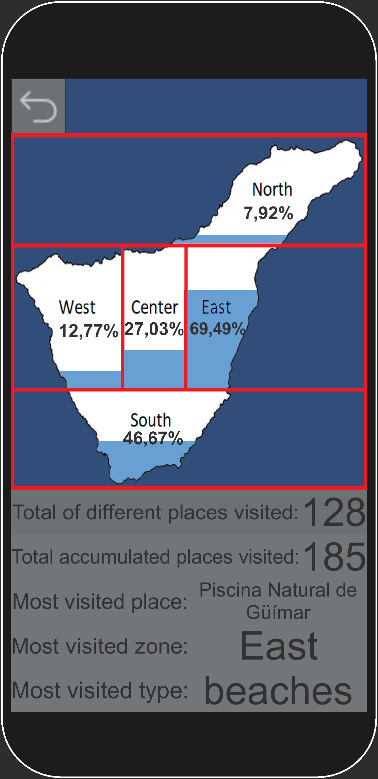
\includegraphics[width=0.25\textwidth]{Memoria_TFG_LaTeX/images/pantallaEstadisticas.png}
    \caption{Pantalla de las estadísticas ejecutándose en un emulador}
    \label{fig:pantallaEstadísticas}
\end{figure}

\newpage
\section{Recompensas}
\subsection{Rangos por nivel}
Los rangos de nivel dentro de la aplicación también presentan una forma de recompensar al usuario, haciéndole conocedor de su progreso gracias a la distinción de otros usuarios con menor rango.
Para establecer los rangos de nivel dentro de la aplicación se han utilizado los nombres de los diferentes niveles sociales que tenían los guanches\footnote{\textbf{Guanches}: Guanche es el nombre que se aplica a los antiguos aborígenes de la isla de Tenerife, Canarias, España, quienes la habitaban antes de la conquista castellana en 1496. Se trata de uno de los pueblos aborígenes de Canarias entroncados genética y culturalmente con los bereberes del norte de África.}.

La sociedad guanche era patriarcal\cite{sociedadguanche}, dividida en grupos sociales definidos por la riqueza, fundamentalmente la tierra y el ganado, en Tenerife existía una nobleza aborigen que está compuesta por:
\begin{itemize}
\item \textbf{Mencey} rey o monarca de cada uno de los territorios de la Isla o de la Isla entera.
\item \textbf{Achimencey} o gobernador, noble conformado en castas privilegiadas tanto en el ámbito político como religioso, participa en la toma de decisiones del gobierno.
\item \textbf{Guañameñes} o Guadameñas, sumos sacerdotes de los Menceyatos.
\item \textbf{Tagoreros} o Chaureros, corregidores y administradores de los diferentes Auchones.
\item \textbf{Sigoñes} o capitanes.
\item \textbf{Cichiciquitzos} o los guerreros, destinados al manejo de las armas.
\item \textbf{Achicaxna} o personal dedicado a la ganadería y la agricultura.
\item \textbf{Achicaxnais} dedicados a las tareas domésticas (Molineros, pescadores, alfareros, etc.). 
\item Embalsamadores, carniceros y mujeres eran las clases más bajas por su relación con la sangre.\cite{pou2017carniceros}
\end{itemize}

Siguiendo esta escala social he diseñado una serie de rangos diferenciados por puntuación:

\begin{ThreePartTable}
\label{table:rangos}
\captionof{table}{Puntos necesarios para alcanzar cada uno de los rangos}

\begin{tabularx}{0.9\textwidth} { 
  | >{\raggedright\arraybackslash}X
  | >{\raggedright\arraybackslash}X
  | >{\raggedright\arraybackslash}X
  | >{\raggedleft\arraybackslash}X | }
    \hline \textbf{Nombre Rango} & \textbf{Puntuación mínima}\\
    \hline Mencey                &  50.000\\
    \hline Achimencey            &  10.000\\
    \hline Guañameñe             &   3.000\\
    \hline Tagorero              &   1.500\\
    \hline Sigoñes               &     750\\
    \hline Cichiciquitzos        &     300\\
    \hline Achicaxna             &     100\\
    \hline Achicaxnais           &       0\\
    \hline 
\end{tabularx}
\end{ThreePartTable}
\begin{figure}[H]
    \centering
    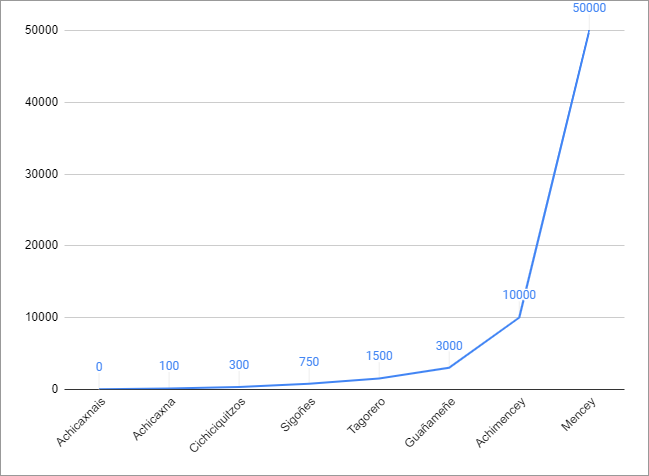
\includegraphics[width=1\textwidth]{Memoria_TFG_LaTeX/images/rangosGrafico.png}
    \caption{Diagrama que muestra el incremento de la puntuación requerida para pertenecer a un rango}
    \label{fig:puntosPorRango}
\end{figure}

Hay que destacar que, en el diseño de rangos, se ha buscado hacer que los rangos más bajos estén menos distanciados en cuanto a puntuación. Esto es así para hacer que los usuarios nuevos sientan que están progresando rápidamente cuando llevan poco tiempo usando la aplicación, de esta manera se consigue que los usuarios se familiaricen rápidamente con el sistema de rangos y, además, sientan cierta satisfacción por el rápido ascenso. Progresivamente, los siguientes rangos se van distanciando para hacer que, para los jugadores veteranos, siga siendo un reto moderadamente difícil e interesante subir de rango.


%%%%%%%%%%%%%%%%%%%%%%%%%%%%%%%%%%%%%%%%%%%%%%%%%%%%%%%%%%%%%%%%%%%%%%%%%%%%%%%
\newpage{\pagestyle{empty}}
\thispagestyle{empty}

\chapter{\LARGE Estudio de viabilidad económica del proyecto}
\label{chapter:viabilidad}

En este capítulo se describirá el análisis económico que se ha llevado a cabo para determinar la viabilidad del desarrollo de este proyecto de manera profesional.

\section{Fuentes de ingreso}
Las posibles fuentes de ingreso que se han barajado se describen en la siguiente lista:
\begin{itemize}
\item \textbf{Vender la propia app}: La solución más obvia, pero quizás no la mejor, es simplemente vender la aplicación en las tiendas digitales para móviles como Google Play Store o su equivalente en iOS, Apple Store. La barrera de tener que pagar para probar la aplicación podría reducir considerablemente el número de usuarios que participarían en la aplicación.

\item \textbf{Google ads}: Una manera de generar ingresos podría ser incluir Google Ads a la aplicación. De esta manera no perderíamos cuota de usuarios y generaríamos unos ingresos proporcionales a la cantidad de usuarios que la utilicen. Además, esta opción cuenta con otra ventaja, y es la de poder dirigir los anuncios en función de la localización del usuario. Pudiendo publicitar lugares que se encuentren físicamente cerca del usuario potenciando los efectos de esta.

\item \textbf{Publicidad de empresas locales}: Esta manera de generar ingresos consistiría en contactar con lugares de ocio de la Isla, como pueden ser centros comerciales, parques de atracciones, zoológicos, actividades, etc. O incluso, de gastronomía, como restaurantes de comida típica canaria. Y colocarlos como punto de interés dentro del mapa de la aplicación, por lo que los usuarios verían ese punto en el catálogo de lugares y, si quisieran completar el mapa de la Isla deberían, al menos, acercarse al lugar. Esto podría ser un incentivo más para que los usuarios visiten esos lugares de ocio y posiblemente generar ingresos en esos lugares o al menos, aumentar el número de personas que transitan por esa zona. Se podrían establecer contratos temporales con las marcas, y que, al finalizar el contrato, ese punto de interés desapareciera del mapa del juego.

\item \textbf{Subvención del Gobierno o del Cabildo}: Quizás sería posible contactar con el Gobierno o el Cabildo de Canarias para ofrecerles participar en el proyecto para fomentar el turismo en la Isla. También se podría exportar fácilmente la app a otras Islas o simplificarla haciendo, por ejemplo, que sea un mapa turístico detallado, de ciudades importantes como Santa Cruz de Tenerife o La Laguna, incluyendo plazas, monumentos históricos, esculturas, etc.
\end{itemize}

Cabe destacar, que se podría hacer una combinación de estas soluciones, es decir, podríamos tener la app con publicidad de Google Ads y con lugares promocionados y ofrecer a los usuarios una versión "premium" sin publicidad.

\section{Desarrollo del proyecto}

En esta sección responderemos a las preguntas: ¿Cuánto cuesta desarrollar este proyecto? ¿Cuánto tiempo tardaría en llevarse a cabo de forma profesional el proyecto? ¿Cuándo se recuperaría la inversión inicial?

Para responder estas preguntas he utilizado el software ProjectLibre\footnote{\textbf{ProjectLibre}: es un software de administración de proyectos de código abierto programado en Java.}, done he creado un proyecto, y añadiendo, los costes estimados y la duración estimada de cada tarea se ha calculado la duración estimada del proyecto, el costo estimado y el camino crítico\footnote{\textbf{Camino crítico}: es la sucesión de tareas que marcan el inicio y el fin del proyecto, por lo tanto, son las tareas que siempre que se retrasen producirán un retraso en la fecha de finalización del proyecto.} de este\footnote{Si desea leer con mayor detenimiento la estructuración de las tareas que componen el proyecto, el archivo que las contiene está disponible en el \href{https://github.com/AaronJoseCabreraMartin/TFG-DiscoverTenerife}{GitHub del proyecto}}.

El proyecto ha sido planteado para estar dividido en cuatro etapas:
\begin{itemize}
\item \textbf{Análisis}: En esta primera etapa se llevará a cabo un estudio de mercado en el que se incluirán tareas como: desarrollo de un análisis PEST, un análisis DAFO, un estudio sobre la identificación de la competencia y un estudio de perfiles de usuarios. También se realizará un diagrama de casos de uso UML y, para finalizar esta etapa, la creación de un documento de análisis de requerimientos. Esta etapa durará un total de 45 días.

\item \textbf{Diseño}: En esta segunda etapa se realizará el diseño completo de la base de datos, la elección del hardware y software a utilizar durante el proyecto y, por último, el diseño de las reglas del juego; cuánta puntuación se obtiene por visitar un lugar, cuánta puntuación se obtiene  por completar un reto, etc. Esta etapa durará un total de 8 días.

\item \textbf{Desarrollo}: Esta segunda etapa es la más se alarga en el tiempo de todo el proyecto. En esta etapa se implementará el diseño de la base de datos realizado en el apartado anterior, se realizará todo el proceso de extracción de información de la web: creando el web scraper, realizando una limpieza de los datos obtenidos y subiendo la información correctamente estructurada a la base de datos. También se realizará el diseño de la interfaz gráfica tanto de la página web como de la aplicación móvil. Y, la última parte, la más importante y larga en el tiempo, la creación de la página web y de la aplicación. Esta etapa dura un total de 65 días.

\item \textbf{Despliegue}: En esta última etapa se incluye la fase de pruebas intensivas a los cuatro sectores del proyecto, al servidor, a la página web, a la aplicación de Android y a la aplicación de iOS. Además, también se incluye la subida de la aplicación a las plataformas de descarga de aplicaciones anteriormente mencionadas, Google Play Store  y Apple Store, con el consecuente cambio a modo de producción. En este punto el proyecto comienza a generar dinero, pero, también en este punto, se añaden los gastos de producción, como son el mantenimiento de Firebase y el mantenimiento de la aplicación, con actualizaciones que corrijan posibles errores, etcétera.
\end{itemize}

\begin{figure}[H]
    \centering
    \includegraphics[width=1\textwidth]{Memoria_TFG_LaTeX/images/Gantt1AnalisisDiseño.png}
    \caption{Primera parte del diagrama de Gantt. En este se muestran las fases de análisis y diseño}
    \label{fig:ganttAnalisisDiseño}
\end{figure}

\begin{figure}[H]
    \centering
    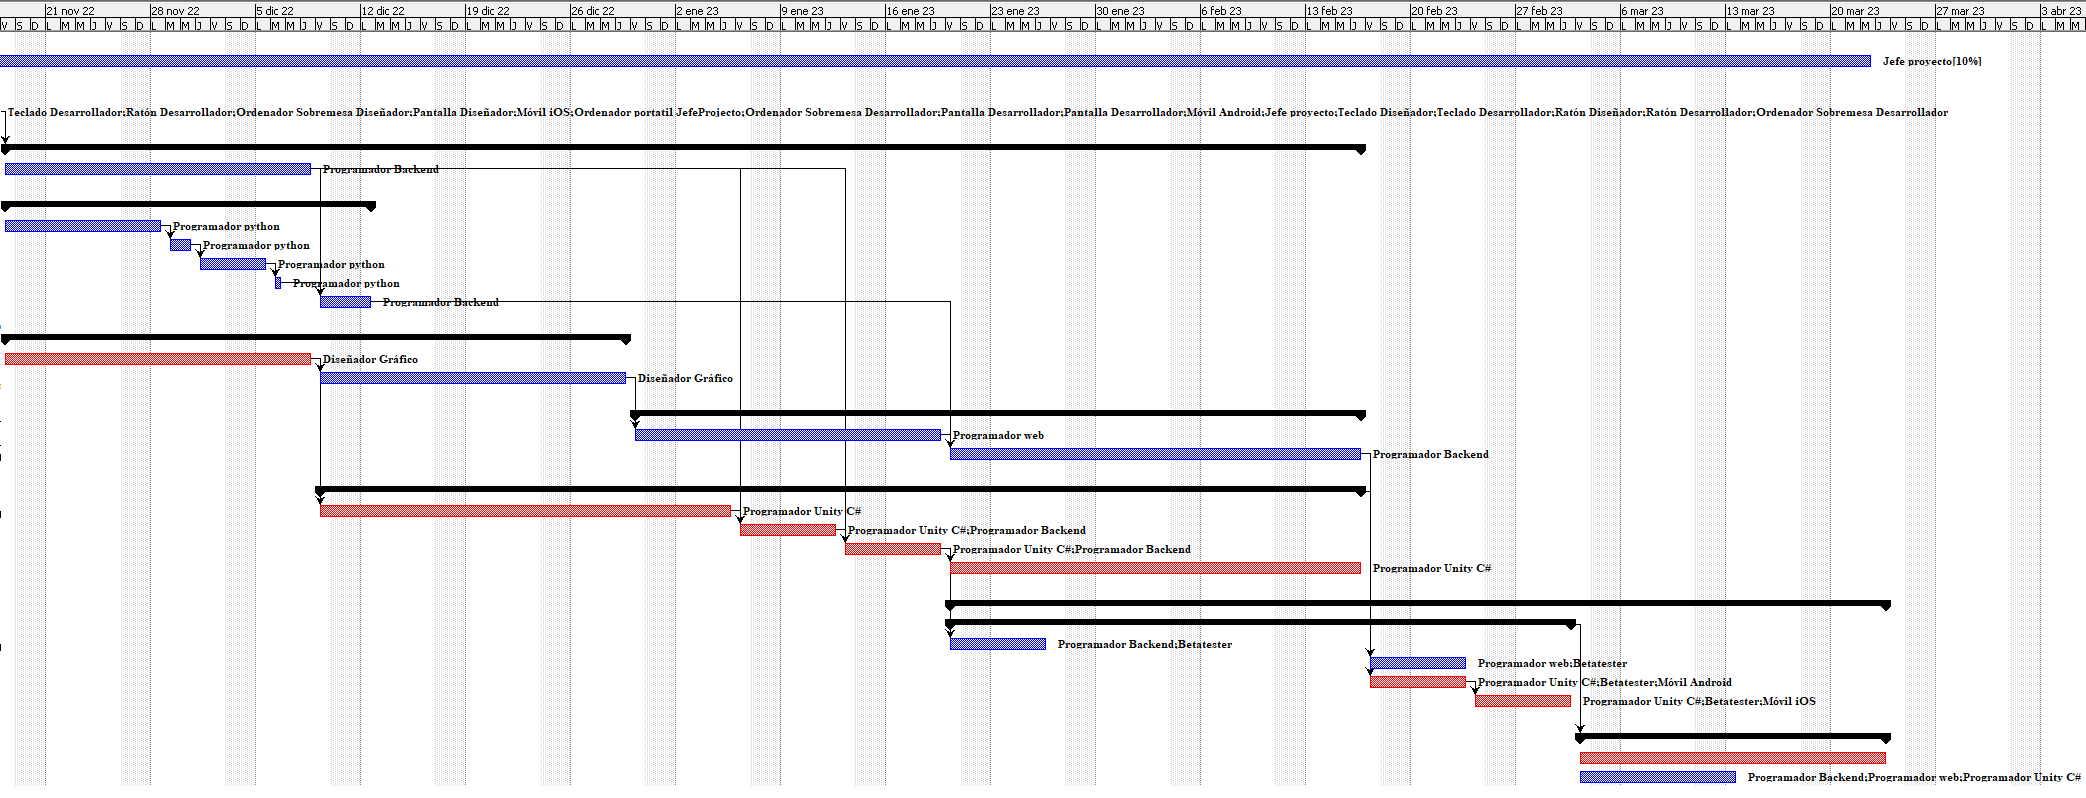
\includegraphics[width=1\textwidth]{Memoria_TFG_LaTeX/images/Gantt2DesarrolloDespliegue.png}
    \caption{Segunda parte del diagrama de Gantt. En este se muestra las fases de desarrollo y despliegue.}
    \label{fig:ganttDesarrolloDespliegue}
\end{figure}

Si se desea observar mejor el diagrama de Gantt o la tabla de recursos, estos están disponibles tanto en forma de imagen como en proyecto de ProjectLibre en el repositorio del proyecto.

\section{Costo y duración del proyecto}

\begin{figure}[H]
    \centering
    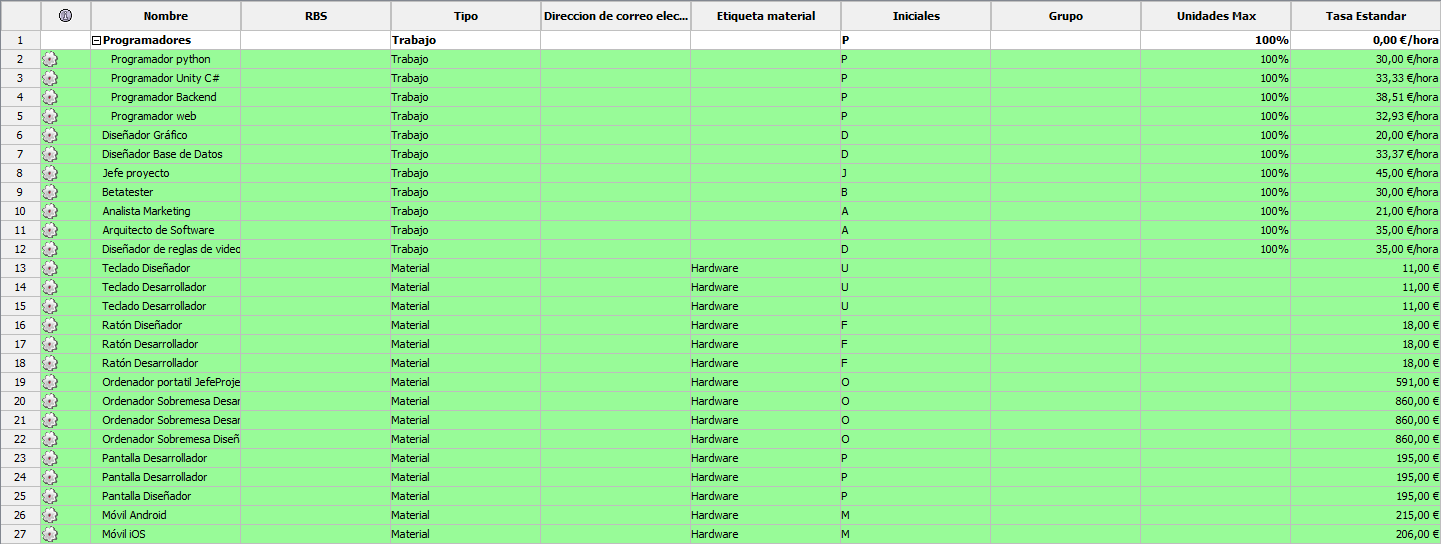
\includegraphics[width=1\textwidth]{Memoria_TFG_LaTeX/images/Recursos.png}
    \caption{Tabla de Recursos tanto materiales como recursos humanos utilizados durante el desarollo del proyecto con sus respectivos costes de uso.}
    \label{fig:tablaRecursos}
\end{figure}

Tras realizar los cálculos de la aproximación de la duración estimada del proyecto, he calculado que el proyecto tardaría 7 meses en terminar su etapa final de creación, el despliegue, y tendría una inversión inicial estimada de, 80569,16 €.

\section{Punto estimado del retorno de la inversión inicial y producción}

En esta fase del proyecto, la aplicación ya está en el mercado y se deben añadir los ingresos que se van generando y los costos de mantenimiento de esta, los cuales, no han sido contabilizados en la inversión inicial.

Para llevar a cabo esta aproximación de los ingresos generados y de los costos de mantenimiento, se ha tenido que aproximar la cantidad de usuarios activos semanales de las dos versiones de la aplicación móvil, Android e iOS, y de la página web.



Con el estudio realizado\footnote{Si desea comprobar el estudio realizado se puede comprobar en el siguiente \href{https://docs.google.com/spreadsheets/d/1Xp9dhk1jerlhGhqqkd2Uu2R6KGxOjXPJQnaUy1ktfSA/edit?usp=sharing}{enlace}.}, se ha demostrado que el proyecto alcanzaría su punto ROI\footnote{\textbf{ROI}: Retorno de Inversión, o por sus siglas en inglés Return Of Investment. Es el instante de tiempo en el cual, el dinero invertido en el proyecto se iguala con el dinero generado por el proyecto.} en la semana número 86 desde el paso a producción, es decir, se tardarían unos 22 meses en recuperar la inversión inicial. A partir de ese punto, el proyecto generaría beneficios para sus inversores. 

\begin{figure}[H]
    \centering
    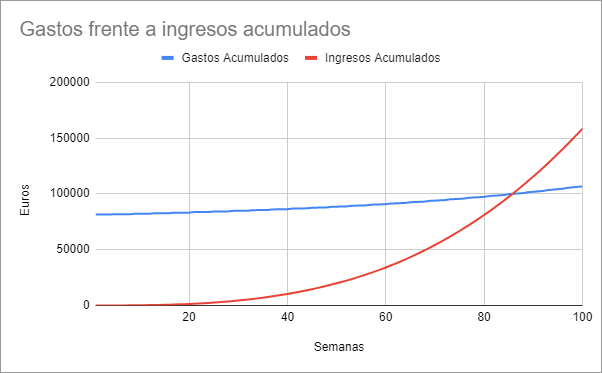
\includegraphics[width=1\textwidth]{Memoria_TFG_LaTeX/images/puntoROI.png}
    \caption{Gráfico en el que se muestra el momento en el cual se alcanza el punto ROI}
    \label{fig:puntoROI}
\end{figure}

Cabe señalar que no se han considerado colaboraciones con empresas locales, establecimientos de interés turístico ni subvenciones del gobierno. Estos ingresos añadidos podrían adelantar en el tiempo el punto ROI.

%%%%%%%%%%%%%%%%%%%%%%%%%%%%%%%%%%%%%%%%%%%%%%%%%%%%%%%%%
\newpage{\pagestyle{empty}}
\thispagestyle{empty}

\chapter{\LARGE Conclusiones y líneas futuras}
\label{chapter:Resultados}

A modo de conclusión, volver a destacar la capacidad que tiene la aplicación de generar economía de kilómetro cero. Pero, no solamente haciendo publicidad de los establecimientos locales, sino que además, se podría integrar un sistema de comentarios o de valoraciones de los establecimientos publicitados, de los lugares naturales o incluso de actividades deportivas como puede ser experiencias con parapentes, etc. Esto generaría una comunidad en la que los usuarios podrían compartir sus experiencias, retar a sus amigos a participar en dichas actividades o visitar esos lugares. Y, al mismo tiempo, generaría retroalimentación para las empresas.

Gracias a la estructura del código, la aplicación podría adaptarse para funcionar con otras Islas o especializarse en ciudades importantes como La Laguna o Santa Cruz de Tenerife, incluyendo información sobre la historia de la ciudad, las plazas, las fuentes, etc.

Para lograr un acabado más profesional, se debería, a la hora de registrarse con cuenta de correo electrónico y contraseña, verificar el correo para evitar denegaciones de servicio. Y además, se podría añadir sistema de verificación en dos pasos y algún método de recuperación de contraseña.

Para añadirle mayor factor de gamificación podríamos establecer ``logros`` por:
\begin{itemize}
\item Ser el primer jugador en visitar un lugar.
\item Visitar cierta cantidad de veces un mismo sitio.
\item Visitar cierta cantidad de veces todos los sitios de la zona o de la Isla.
\item Acumular cierta cantidad de visitas en total de todos los sitios.
\end{itemize}

Otro posible añadido sería que los usuarios podrían tener la opción de enviar fotos y descripciones de lugares que no se encuentren dentro de la aplicación para, tras su revisión, ser añadidos al catálogo de la aplicación.

Como conclusión se puede extraer que durante esta memoria se ha demostrado la viabilidad económica, los múltiples beneficios y el potencial de éxito que posee este proyecto.

%%%%%%%%%%%%%%%%%%%%%%%%%%%%%%%%%%%%%%%%%%%%%%%%%%%%%%%%%
\newpage{\pagestyle{empty}}
\thispagestyle{empty}

\chapter{\LARGE Summary and Conclusions}
\label{chapter:Conclusiones}

Most of the Canarian people need the comeback of the tourist situation of Canary Islands to pre-Covid levels. 
During this study, we have shown how a project of a gamified touristic application could be an incentive to make people move through and discover the whole Tenerife island. We also have shown the feasibility to make a reality this project.

We had made a marketing study and a competition study in order to increase the success probability of the project. Besides, we had created a Gantt diagram that proof that the project's deployment could be completed in 7 months. We, also, had made an approximation of the quantity of user that will use both applications and the web page, and with that approximation we had calculated the profits and the costs of having the application working in production. Thanks to this calculus, we have proved that the return of investment will be reached in a moderate time, 22 months.

As a conclusion, it has to be said that during this study we have demonstrated the viability, the benefits, and the potential of this project.


%%%%%%%%%%%%%%%%%%%%%%%%%%%%%%%%%%%%%%%%%%%%%%%%%%%%%%%%%
\newpage{\pagestyle{empty}}
\thispagestyle{empty}

\chapter{\LARGE Presupuesto}
\label{chapter:presupuesto}

Como ya se ha indicado, el proyecto llevaría 7 meses de desarrollo. La inversión inicial ascendería a un total de, 81429.16 €, cabe recordar, que durante el tiempo de producción también hay gastos debido al mantenimiento del proyecto y que se tardará, aproximadamente, 22 meses en recuperar la inversión inicial más el dinero invertido en el mantenimiento. Además, no se han tenido en cuenta gastos en alquiler de una oficina, mantenimiento de esta ni gastos en contratiempos como reparación de los equipos de la oficina, etcétera. 

Al igual que en la mayoría de proyectos de desarrollo de software, el mayor gasto se ha ido en mano de obra. En la siguiente tabla se reflejan las horas de trabajo que supone cada tarea y el coste en €/h de cada una.
\\
\begin{ThreePartTable}
\label{table:tareas}
\captionof{table}{Gastos derivados de la mano de obra utilizada durante el desarrollo}
\begin{tabularx}{0.9\textwidth} { 
  | >{\raggedright\arraybackslash}X
  | >{\raggedright\arraybackslash}X
  | >{\raggedleft\arraybackslash}X | }
    \hline \textbf{Tareas} & \textbf{Horas de trabajo} & \textbf{Costo}\\
    \hline Análisis & 416 & 3696 €\\
    \hline Diseño & 104 & 3535,68 €\\
    \hline Desarrollo & 1224 & 39203,36 €\\
    \hline Despliegue & 320 & 10324 €\\
    \hline Control proyecto & 116,40 & 4656 €\\
    \hline Total & 2180,40 & 69815,04 €\\
    \hline 
\end{tabularx}
\end{ThreePartTable}

En el siguiente diagrama se muestra la distribución del dinero invertido en mano de obra durante el desarrollo.

\begin{figure}[H]
    \centering
    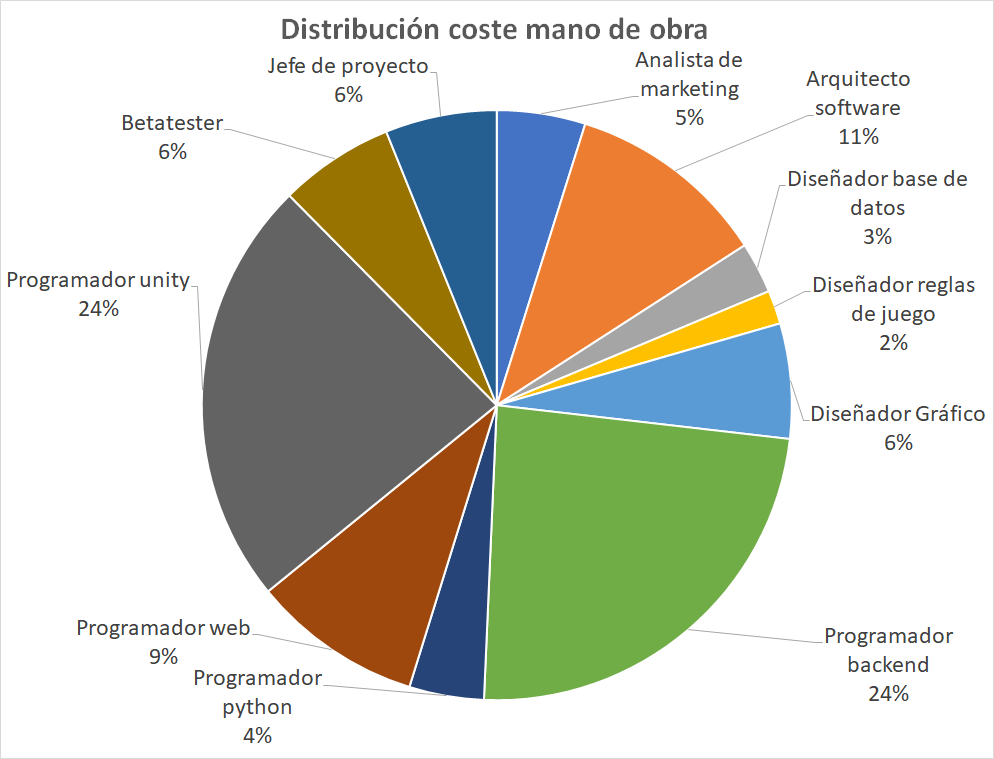
\includegraphics[width=1\textwidth]{Memoria_TFG_LaTeX/images/distribucionGastosManoDeObra.PNG}
    \caption{Distribución de los gastos de la mano de obra durante el desarrollo del proyecto.}
    \label{fig:distribucionGastosManoDeObra}
\end{figure}

El otro gasto que ocurre durante el desarrollo son los gastos en material, en este caso, se tratan de los equipos informáticos de los empleados.

\begin{ThreePartTable}
\label{table:material}
\captionof{table}{Gastos derivados de la compra de hardware durante el desarrollo}

\begin{tabularx}{0.9\textwidth} { 
  | >{\raggedright\arraybackslash}X
  | >{\raggedright\arraybackslash}X
  | >{\raggedright\arraybackslash}X
  | >{\raggedleft\arraybackslash}X | }
    \hline \textbf{Material} & \textbf{Unidades} & \textbf{Costo unidad} & \textbf{Costo}\\
    \hline Teclado & 3 & 11 € & 33 €\\
    \hline Ratón & 3 & 18 € & 54 €\\
    \hline Ordenador Sobremesa & 3 & 860 € & 2580 €\\
    \hline Ordenador Portátil & 1 & 591 € & 591 €\\
    \hline Pantalla & 3 & 195 € & 585 €\\
    \hline Móvil Android & 1 & 215 € & 215 €\\
    \hline Móvil iOS & 1 & 206 € & 206 €\\
    \hline \textbf{Total} &  &  & \textbf{4264 €}\\
    \hline
\end{tabularx}

\end{ThreePartTable}


Como se mencionó anteriormente, la mayor parte del coste de desarrollo se ha invertido en mano de obra. En el siguiente gráfico se puede observar la gran diferencia entre el gasto de mano de obra y el gasto en material.
\begin{figure}[H]
    \centering
    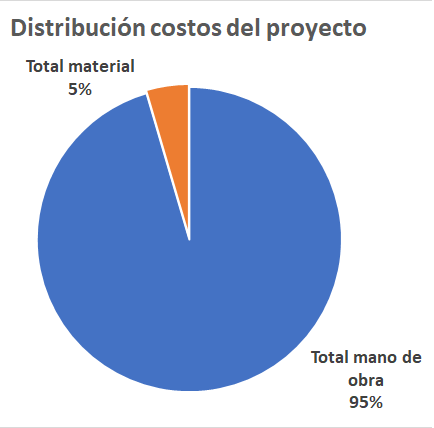
\includegraphics[width=0.75\textwidth]{Memoria_TFG_LaTeX/images/distribucionGastosDesarrollo.PNG}
    \caption{Distribución de los gastos durante el desarrollo del proyecto.}
    \label{fig:distribucionGastosDesarrollo}
\end{figure}

%%%%%%%%%%%%%%%%%%%%%%%%%%%%%%%%%%%%%%%%%%%%%%%%%%%%%%%%%
%\newpage{\pagestyle{empty}\cleardoublepage}
%\thispagestyle{empty}

%\begin{appendix}

%\chapter{\LARGE Título del Apéndice 1}
%\label{appendix:1}
%\section{Algoritmo XXX}
\label{Apendice1:XXX}

\begin{center}
\begin{footnotesize}
\begin{verbatim}

/***********************************************************************************
*
* Fichero .h
*
***********************************************************************************
*
* AUTORES
*   
*
* FECHA
*   
*
* DESCRIPCION
*   
*
************************************************************************************/

\end{verbatim}
\end{footnotesize}
\end{center}

\section{Algoritmo YYY}
\label{Apendice1:YYY}

\begin{center}
\begin{footnotesize}
\begin{verbatim}


/***********************************************************************************
 *
 * Fichero .h
 *
 ***********************************************************************************
 *
 * AUTORES
 *
 * FECHA
 *
 * DESCRIPCION
 *
 *
 ************************************************************************************/
 
\end{verbatim}
\end{footnotesize}
\end{center}

\section{Algoritmo ZZZ}
\label{Apendice1:ZZZ}

\begin{center}
\begin{footnotesize}
\begin{verbatim}


/***********************************************************************************
 *
 * Fichero .h
 *
 ***********************************************************************************
 *
 * AUTORES
 *
 * FECHA
 *
 * DESCRIPCION
 *
 *
 ************************************************************************************/
 
\end{verbatim}
\end{footnotesize}
\end{center}



%\chapter{\LARGE Título del Apéndice 2}
%\label{appendix:2}
%\section{Otro apéndice: Sección 1}
texto

\section{Otro apéndice: Sección 2}
texto

%\end{appendix}

%%%%%%%%%%%%%%%%%%%%%%%%%%%%%%%%%%%%%%%%%%%%%%%%%%%%%%%%%%
% Aquí figurará la bibliografía
\printbibliography
%%%%%%%%%%%%%%%%%%%%%%%%%%%%%%%%%%%%%%%%%%%%%%%%%%%%%%%%%%

\end{document}

